\subsection{Гистограммы и графики плотности распределения}
\begin{figure}[H]
	\centering
	\begin{tabular}{ccc}
		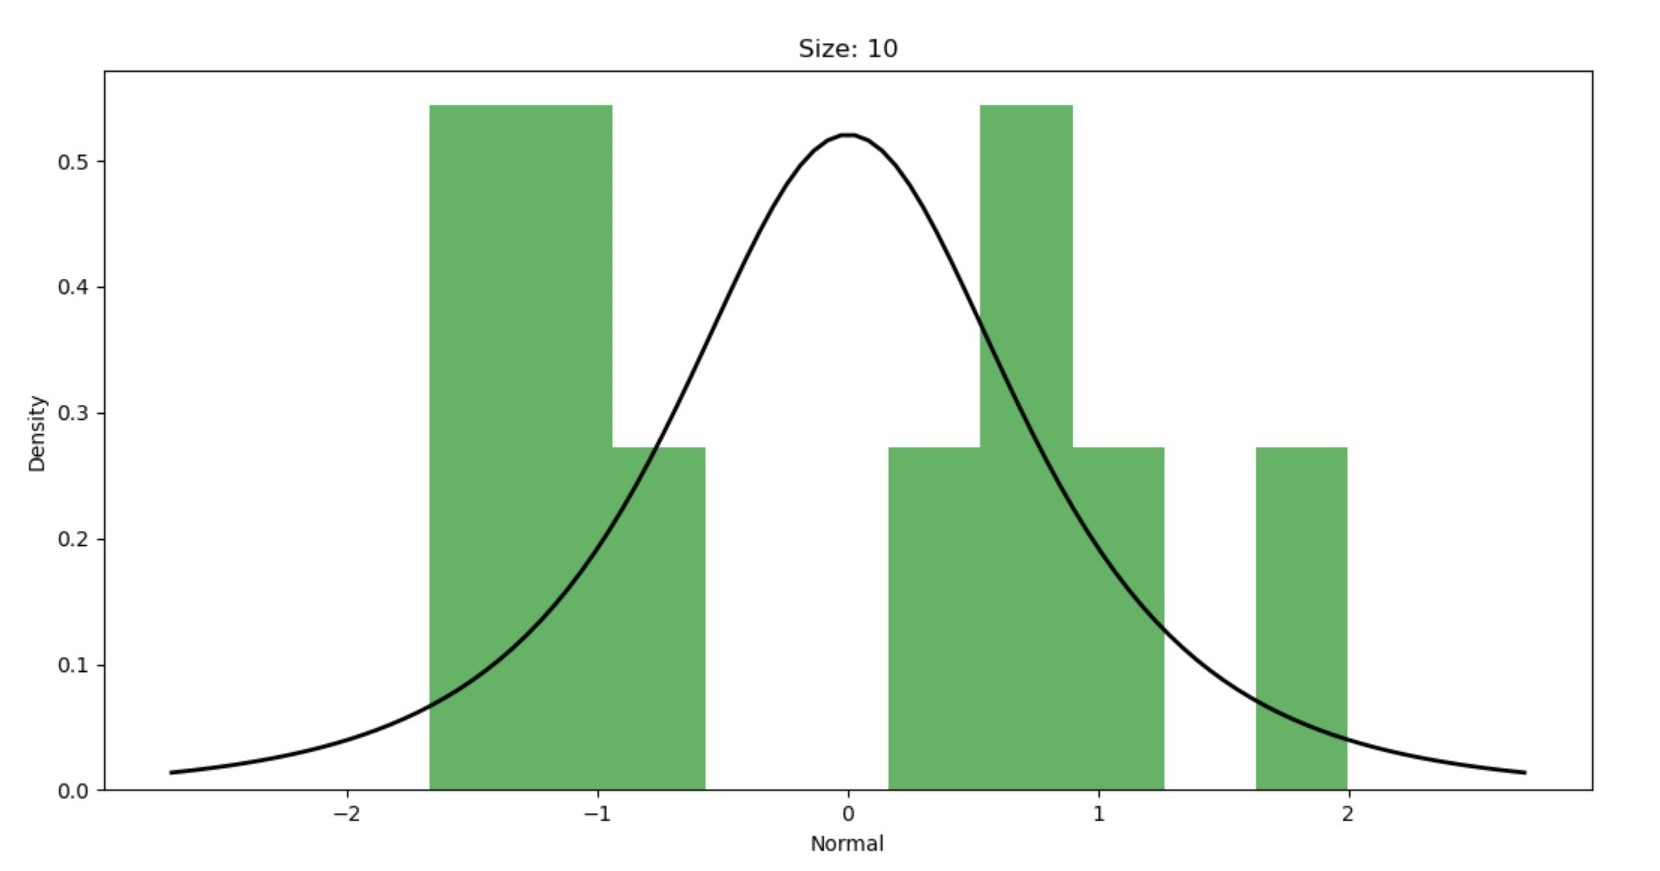
\includegraphics[width=55mm, height =0.25\textheight]{pics/n10.jpg}
		&
		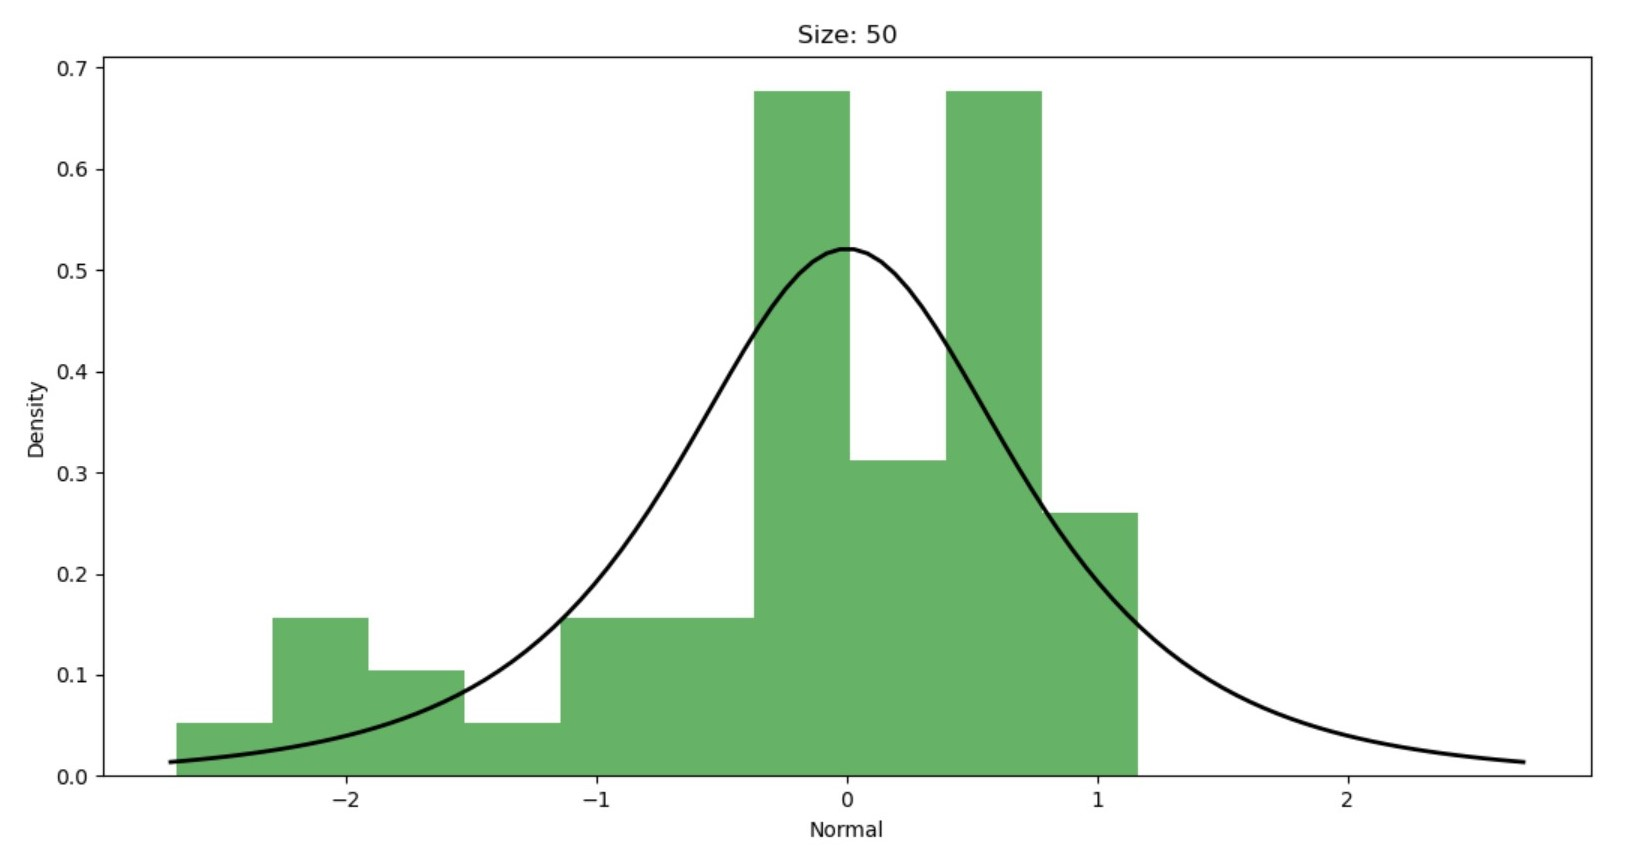
\includegraphics[width=55mm, height =0.25\textheight]{pics/n50.jpg}
		&
		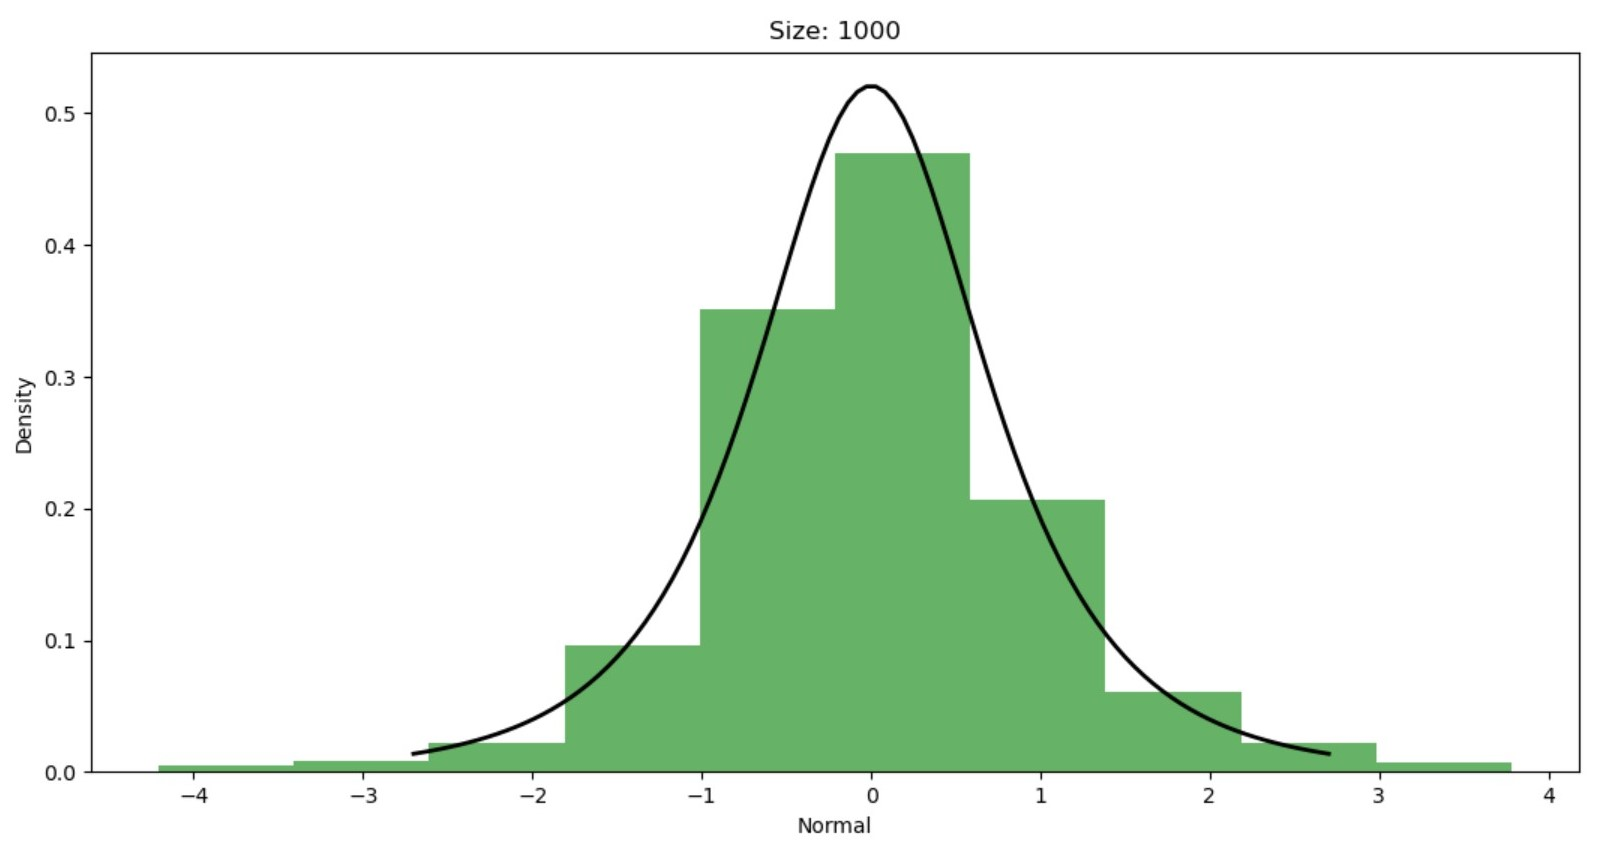
\includegraphics[width=55mm, height =0.25\textheight]{pics/n1000.jpg}
	\end{tabular}
	\caption{Нормальное распределение}
	\label{fig:normal}
\end{figure}

\begin{figure}[H]
	\centering
	\begin{tabular}{ccc}
		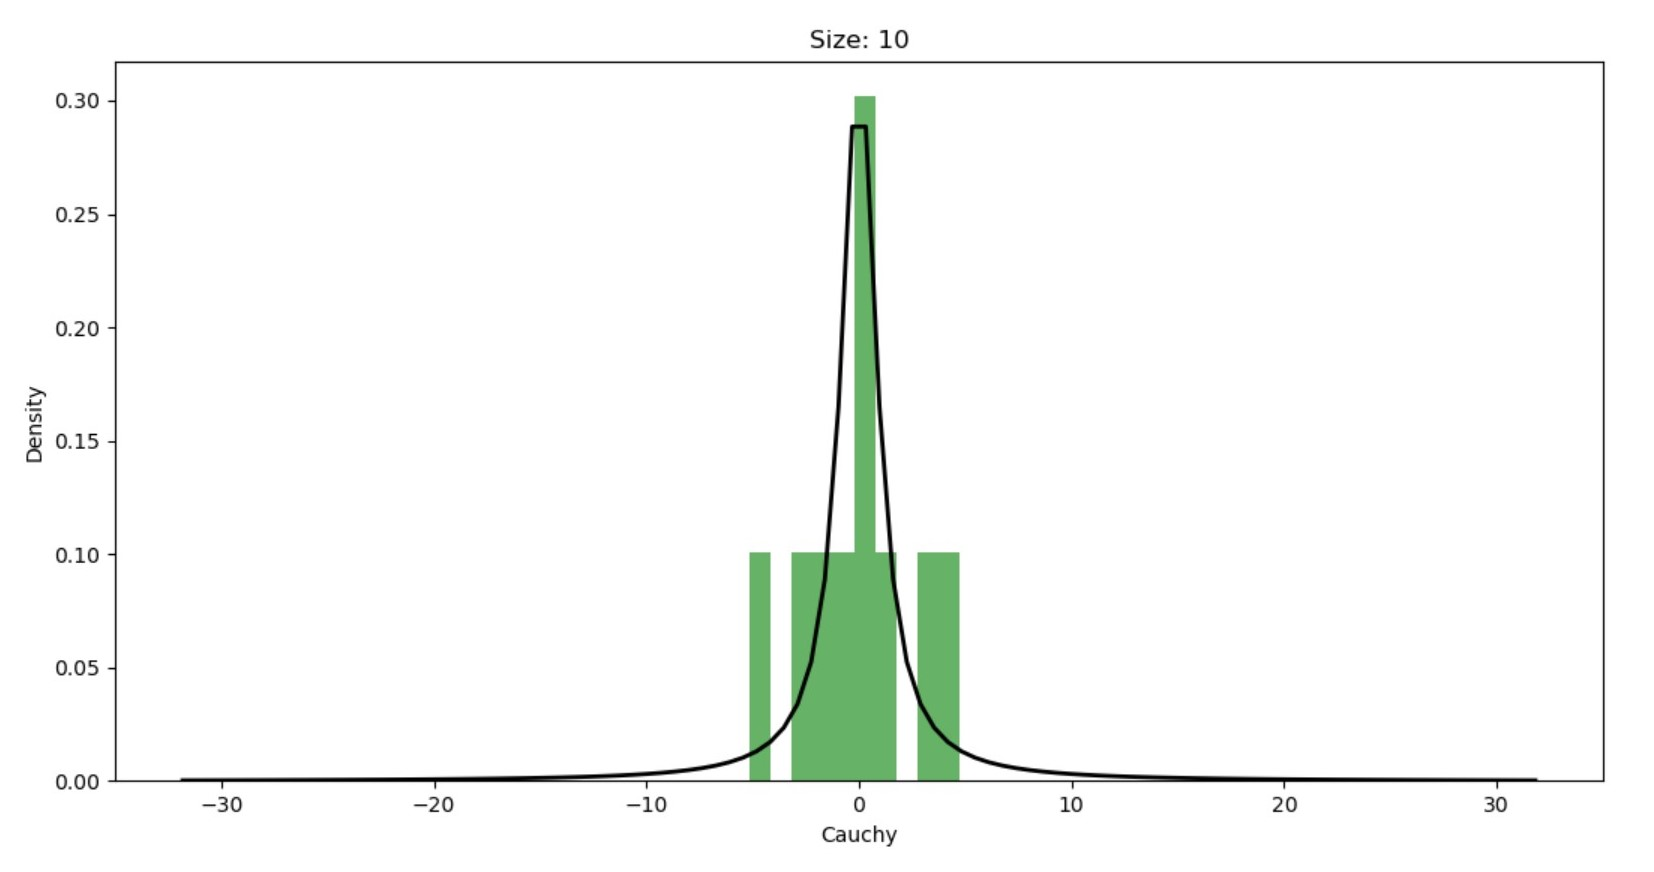
\includegraphics[width=55mm, height =0.25\textheight]{pics/c10.jpg}
		&
		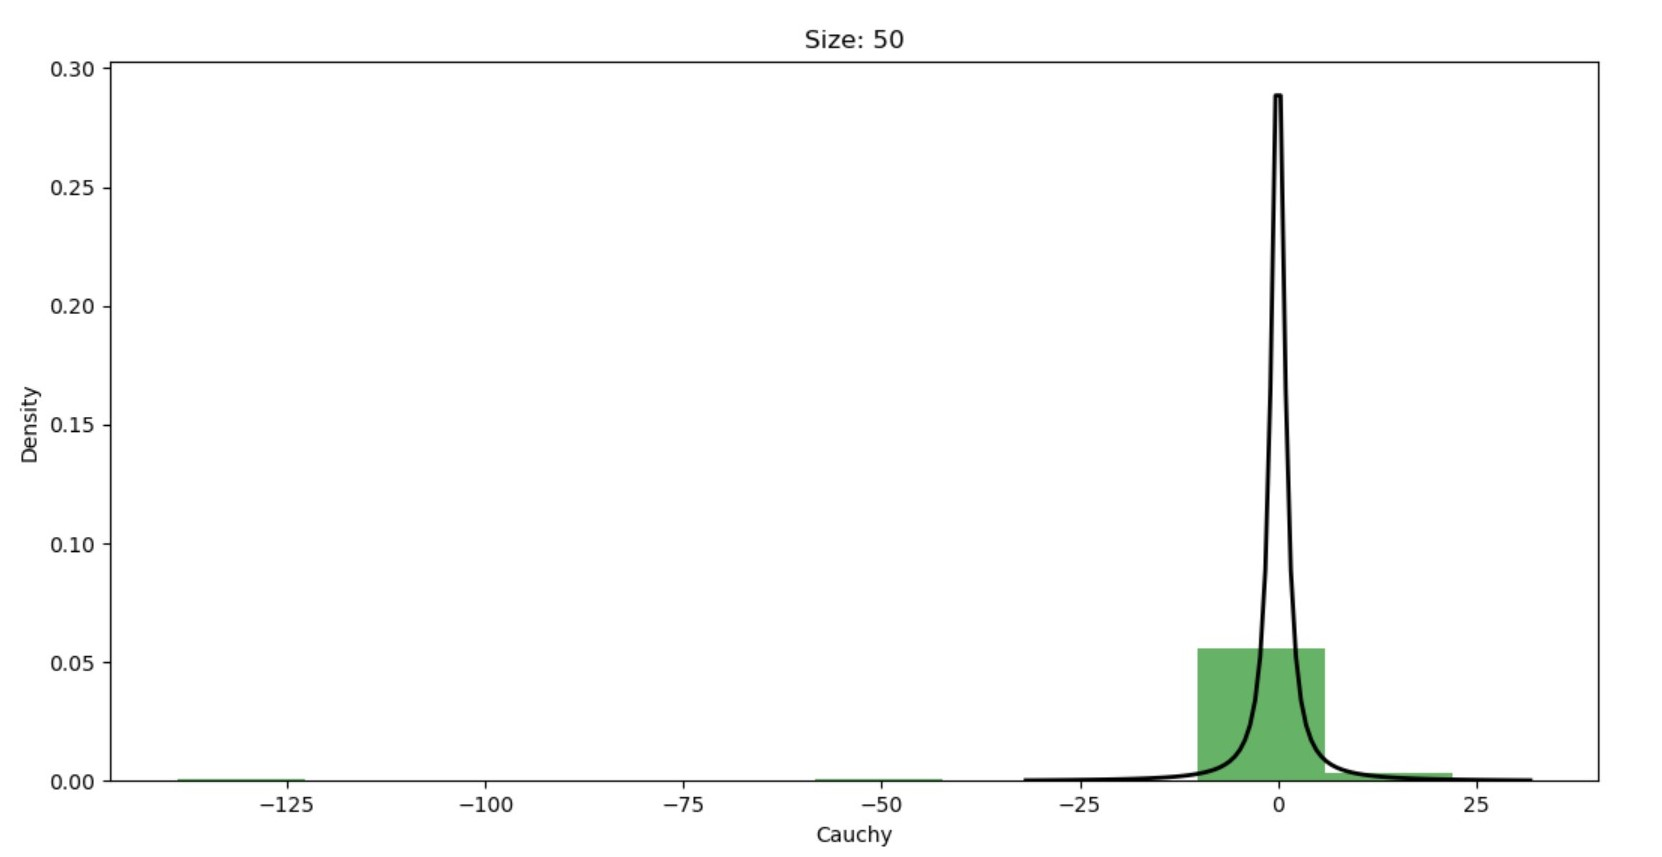
\includegraphics[width=55mm, height =0.25\textheight]{pics/c50.jpg}
		&
		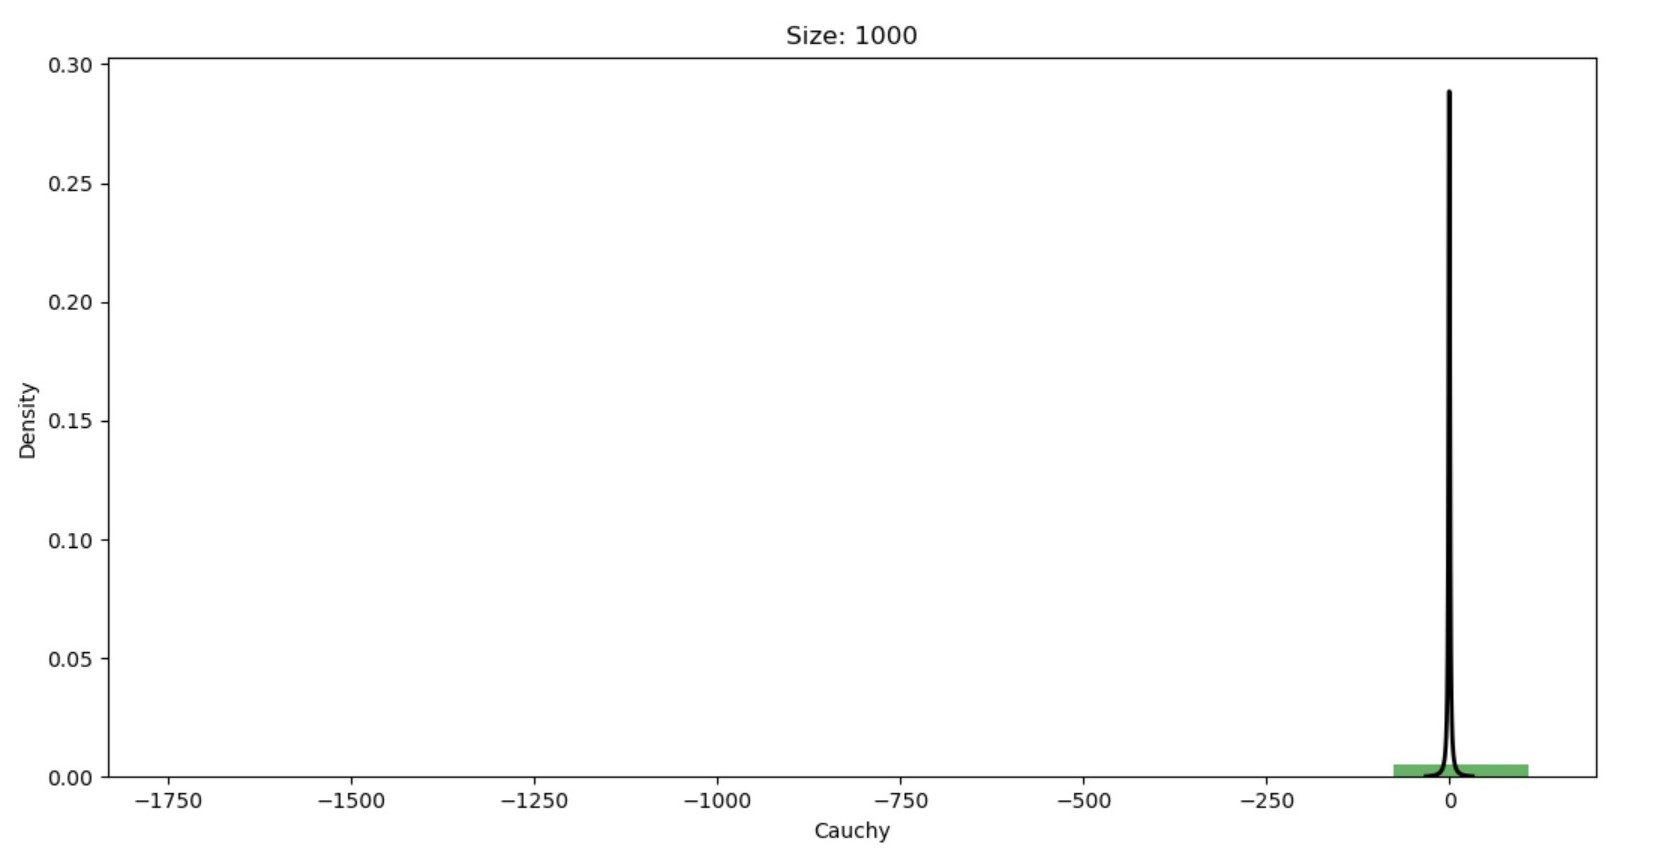
\includegraphics[width=55mm, height =0.25\textheight]{pics/c1000.jpg}
	\end{tabular}
	\caption{Распределение Коши}
	\label{fig:cauchy}
\end{figure}


\begin{figure}[H]
	\centering
	\begin{tabular}{ccc}
		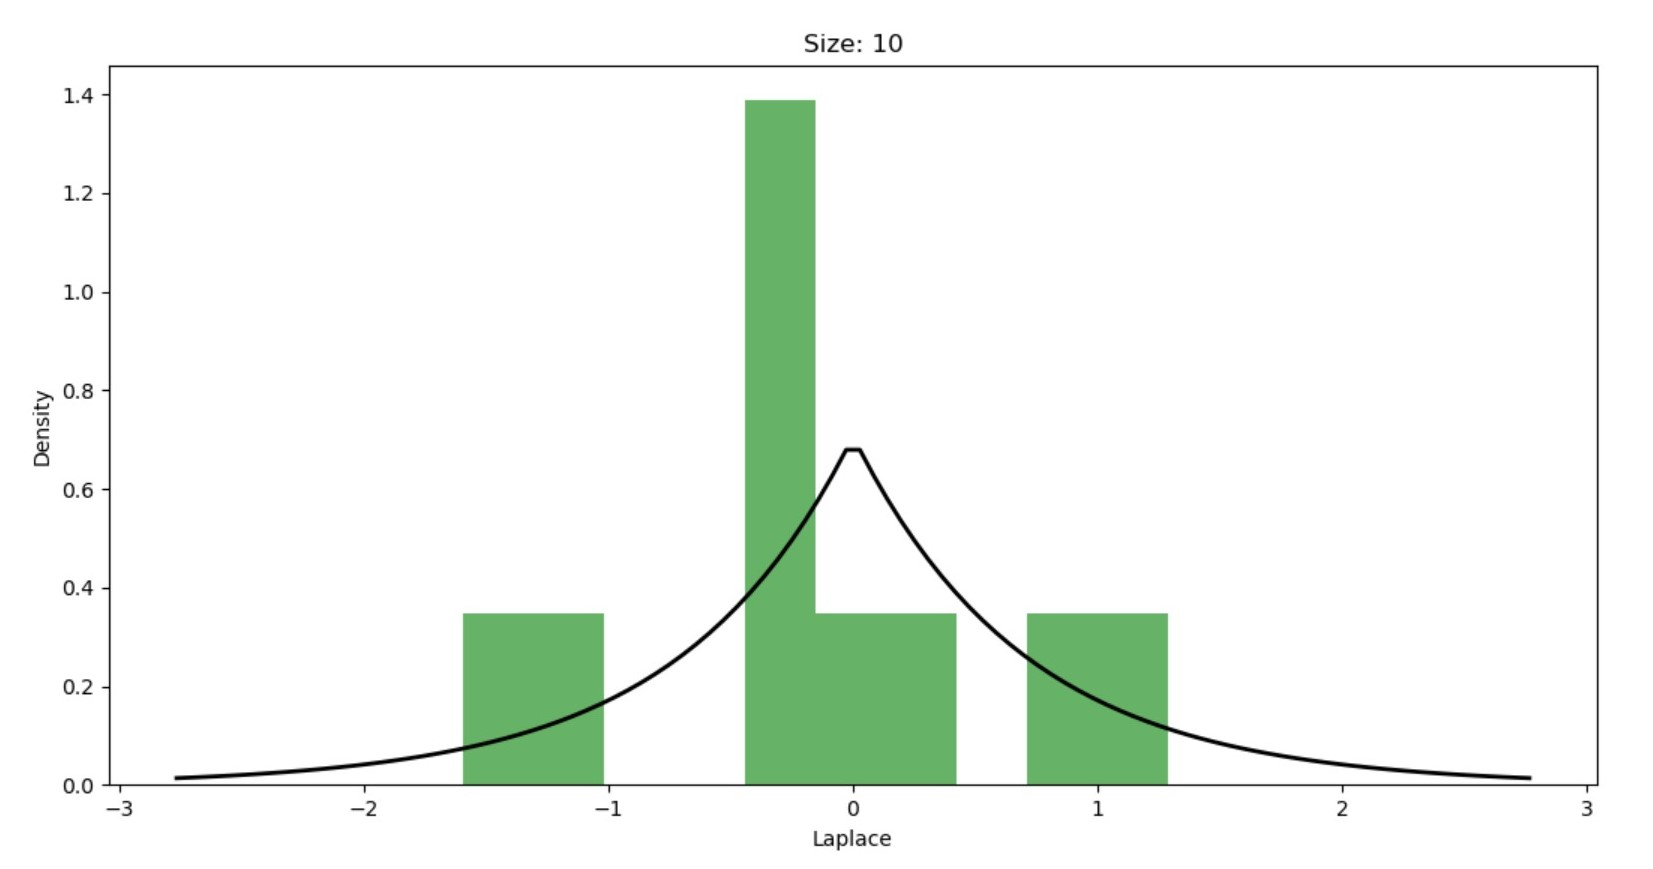
\includegraphics[width=55mm, height =0.25\textheight]{pics/l10.jpg}
		&
		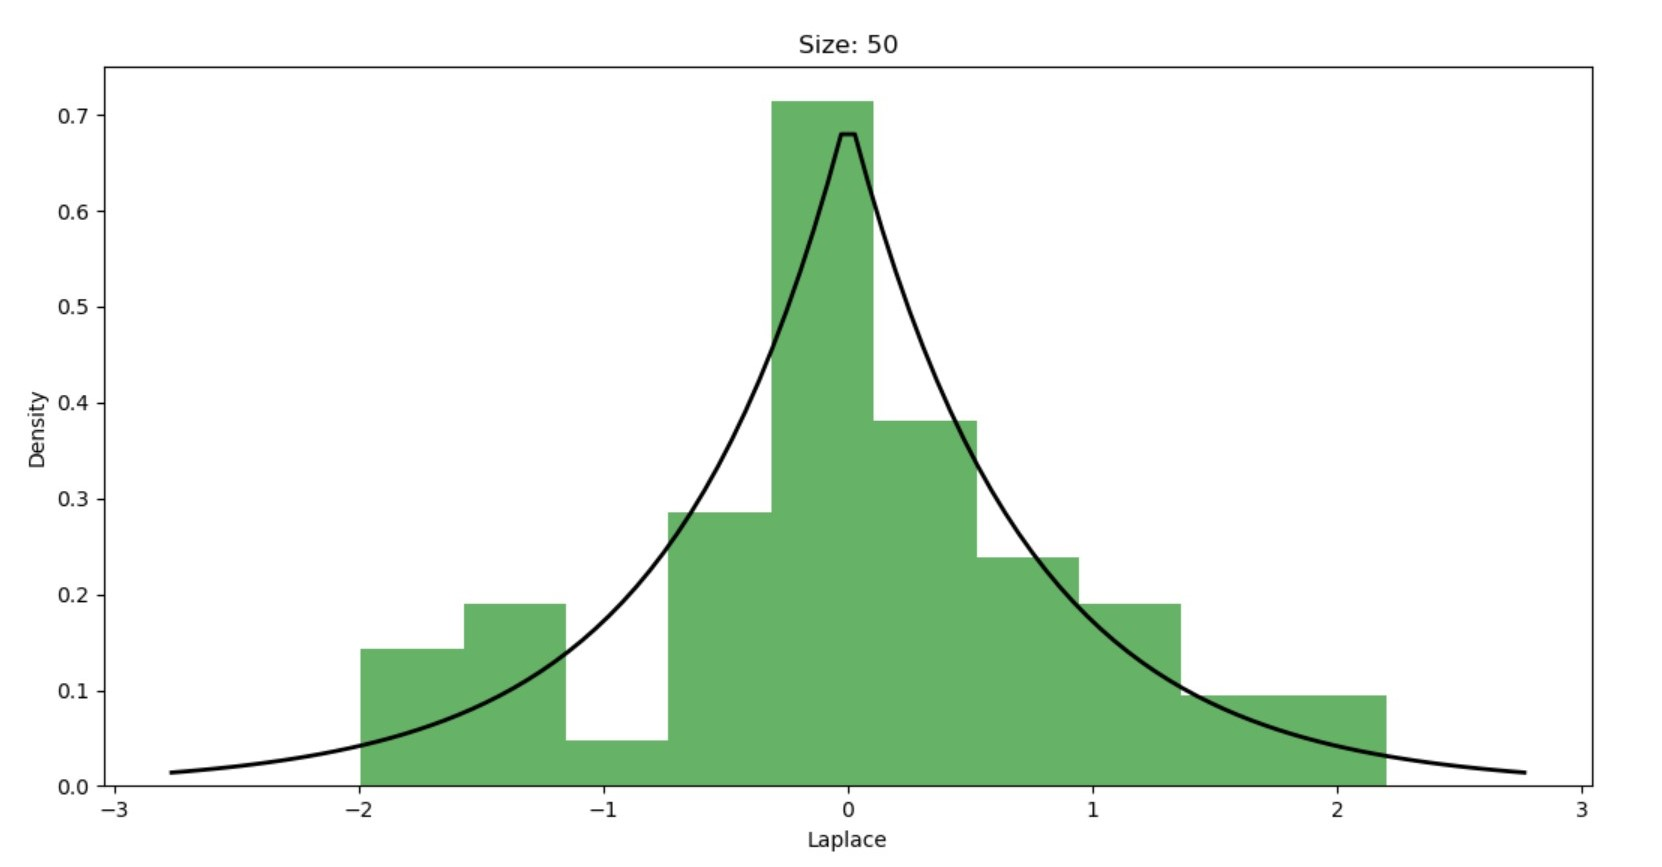
\includegraphics[width=55mm, height =0.25\textheight]{pics/l50.jpg}
		&
		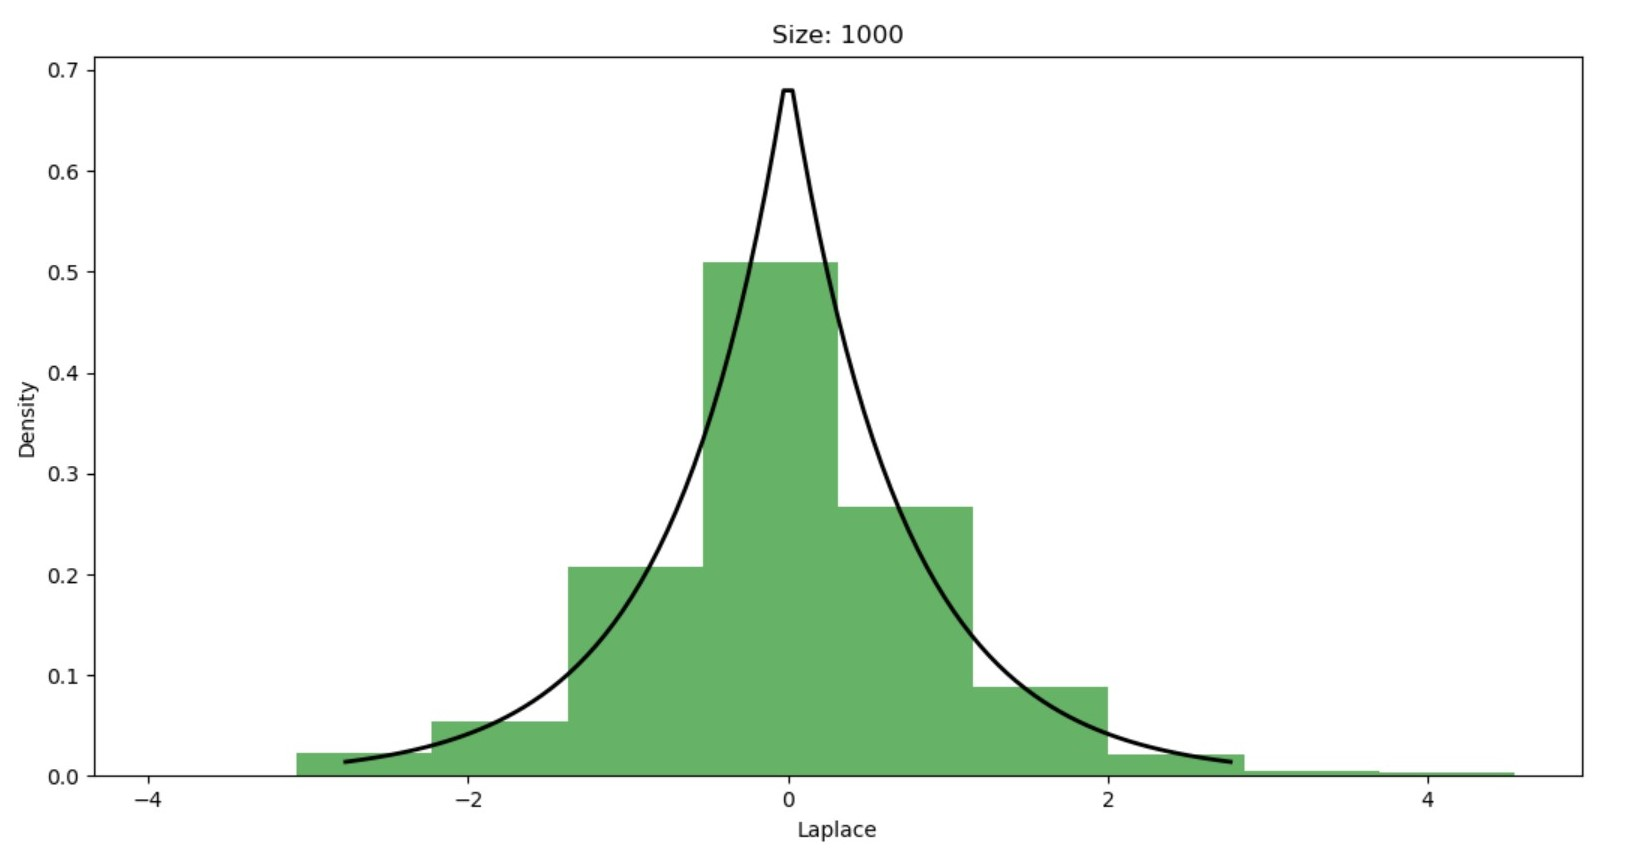
\includegraphics[width=55mm, height =0.25\textheight]{pics/l1000.jpg}
	\end{tabular}
	\caption{Распределение Лапласа}
	\label{fig:laplace}
\end{figure}


\begin{figure}[H]
	\centering
	\begin{tabular}{ccc}
		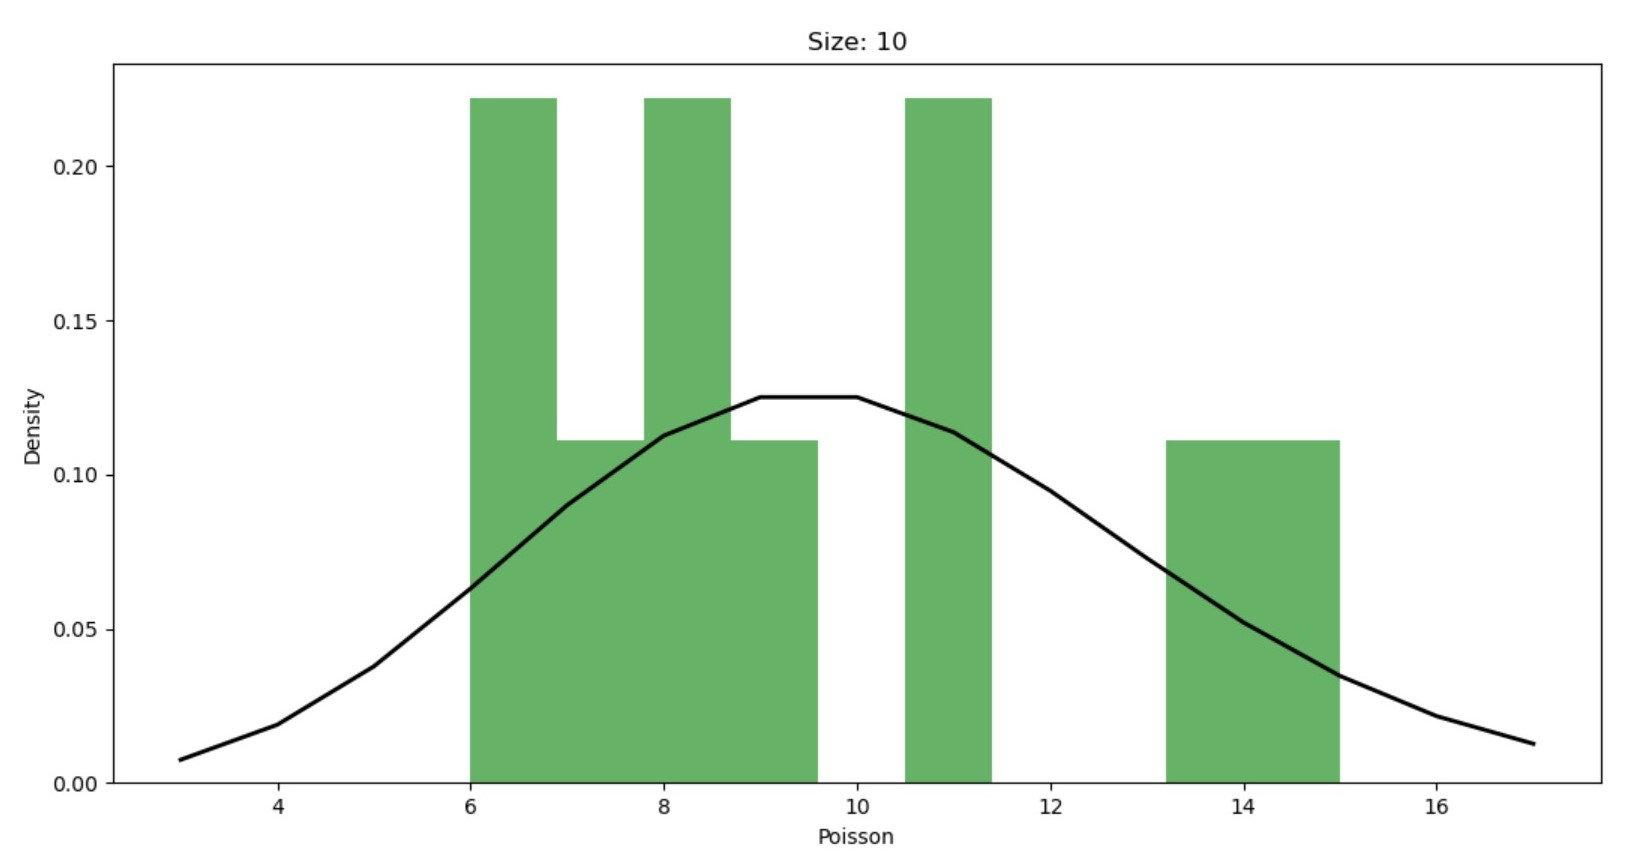
\includegraphics[width=55mm, height =0.25\textheight]{pics/p10.jpg}
		&
		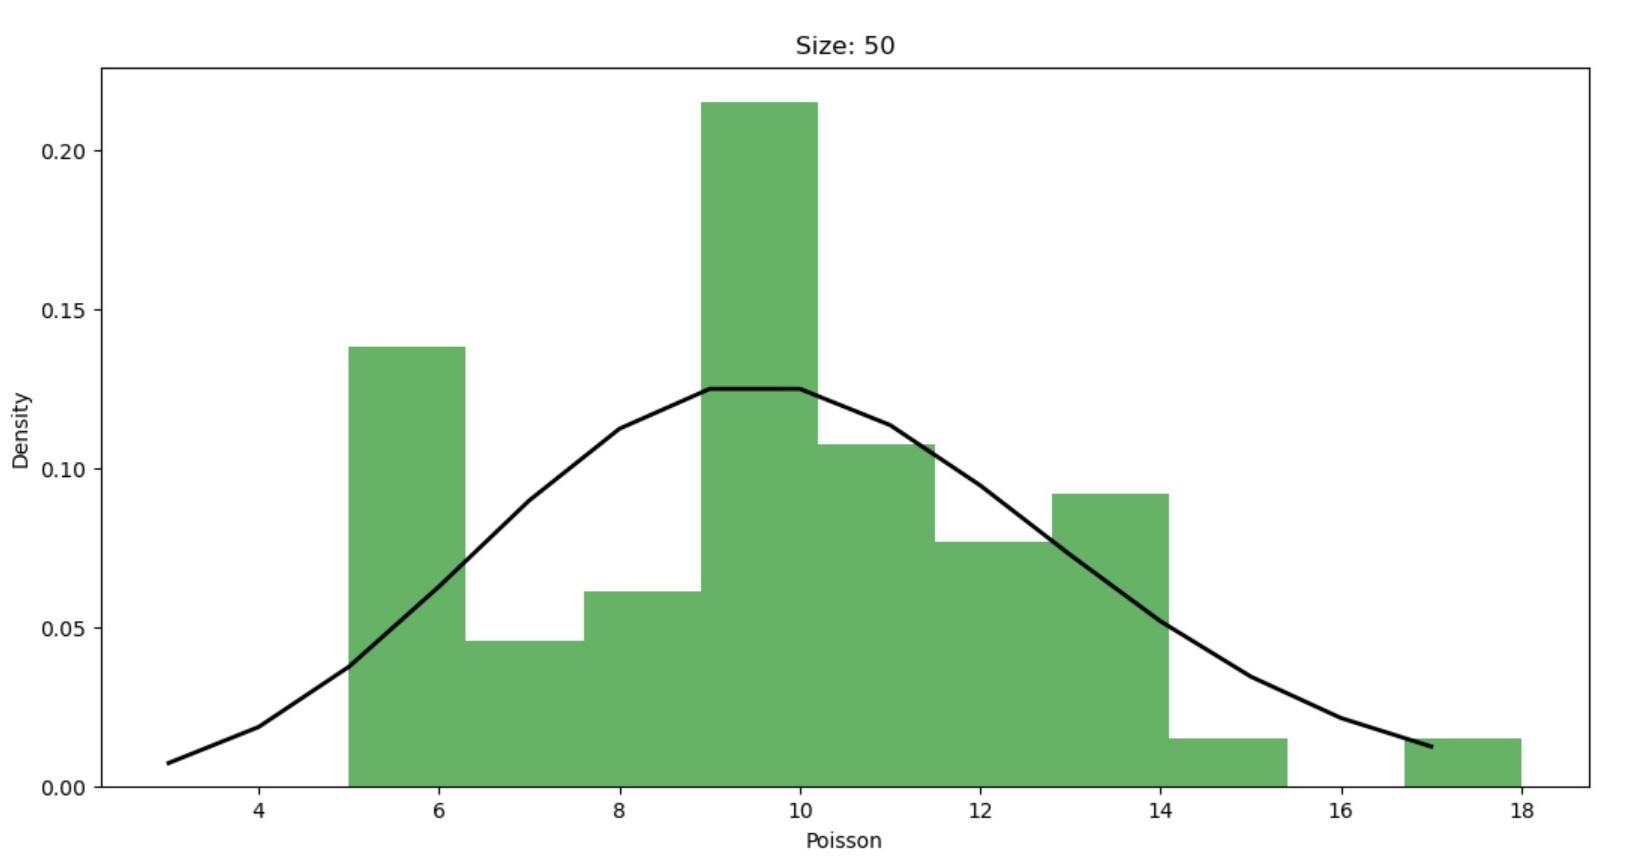
\includegraphics[width=55mm, height =0.25\textheight]{pics/p50.jpg}
		&
		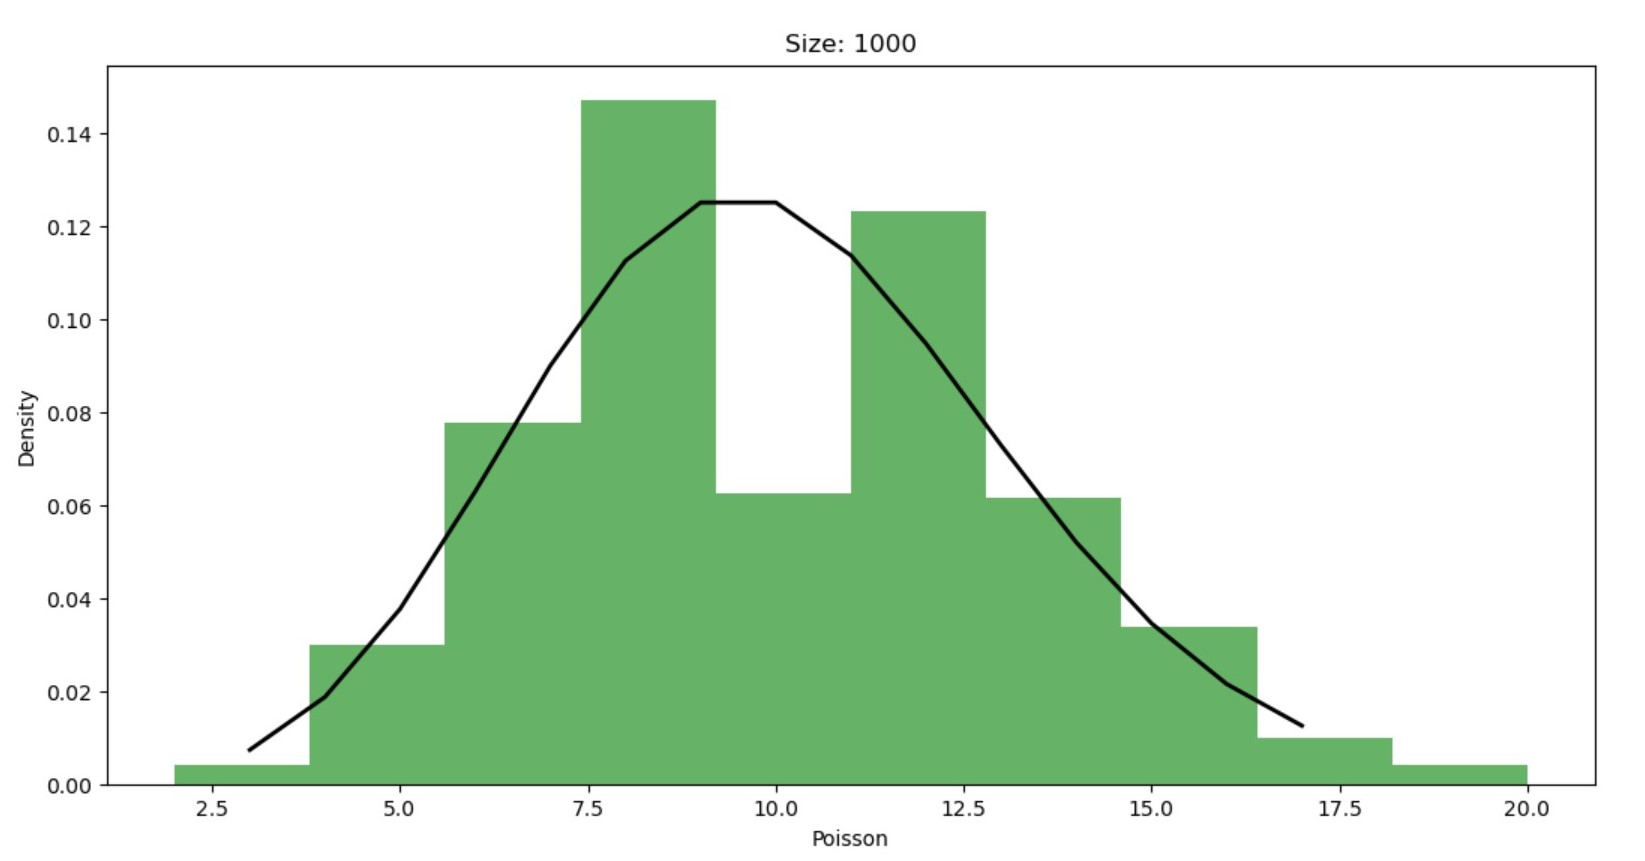
\includegraphics[width=55mm, height =0.25\textheight]{pics/p1000.jpg}
	\end{tabular}
	\caption{Распределение Пуассона}
	\label{fig:poisson}
\end{figure}


\begin{figure}[H]
	\centering
	\begin{tabular}{ccc}
		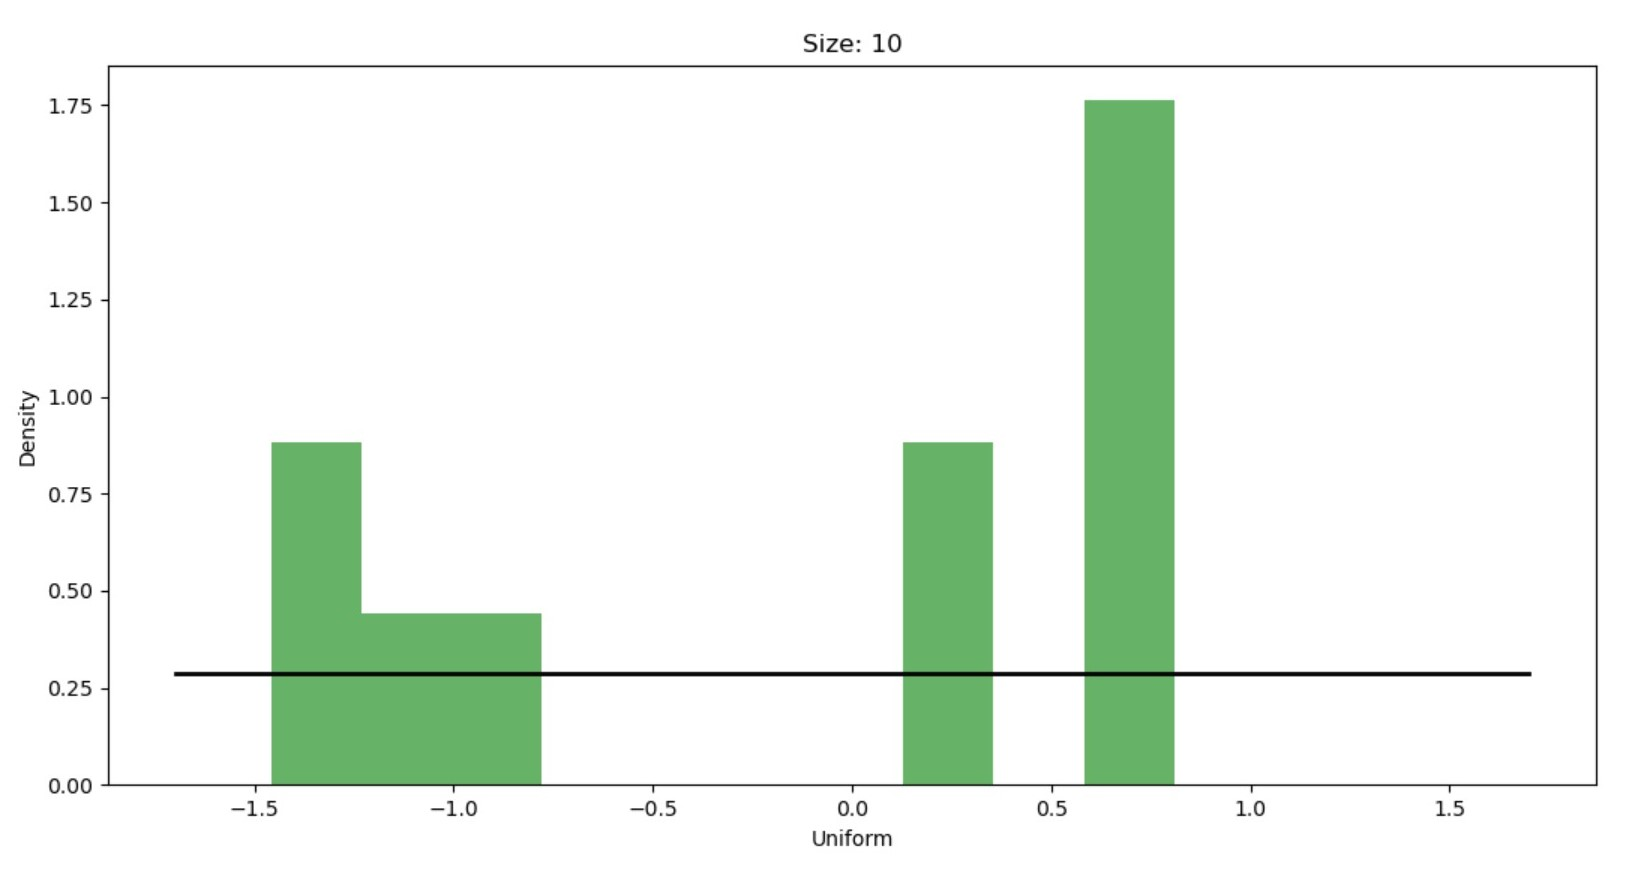
\includegraphics[width=55mm, height =0.25\textheight]{pics/u10.jpg}
		&
		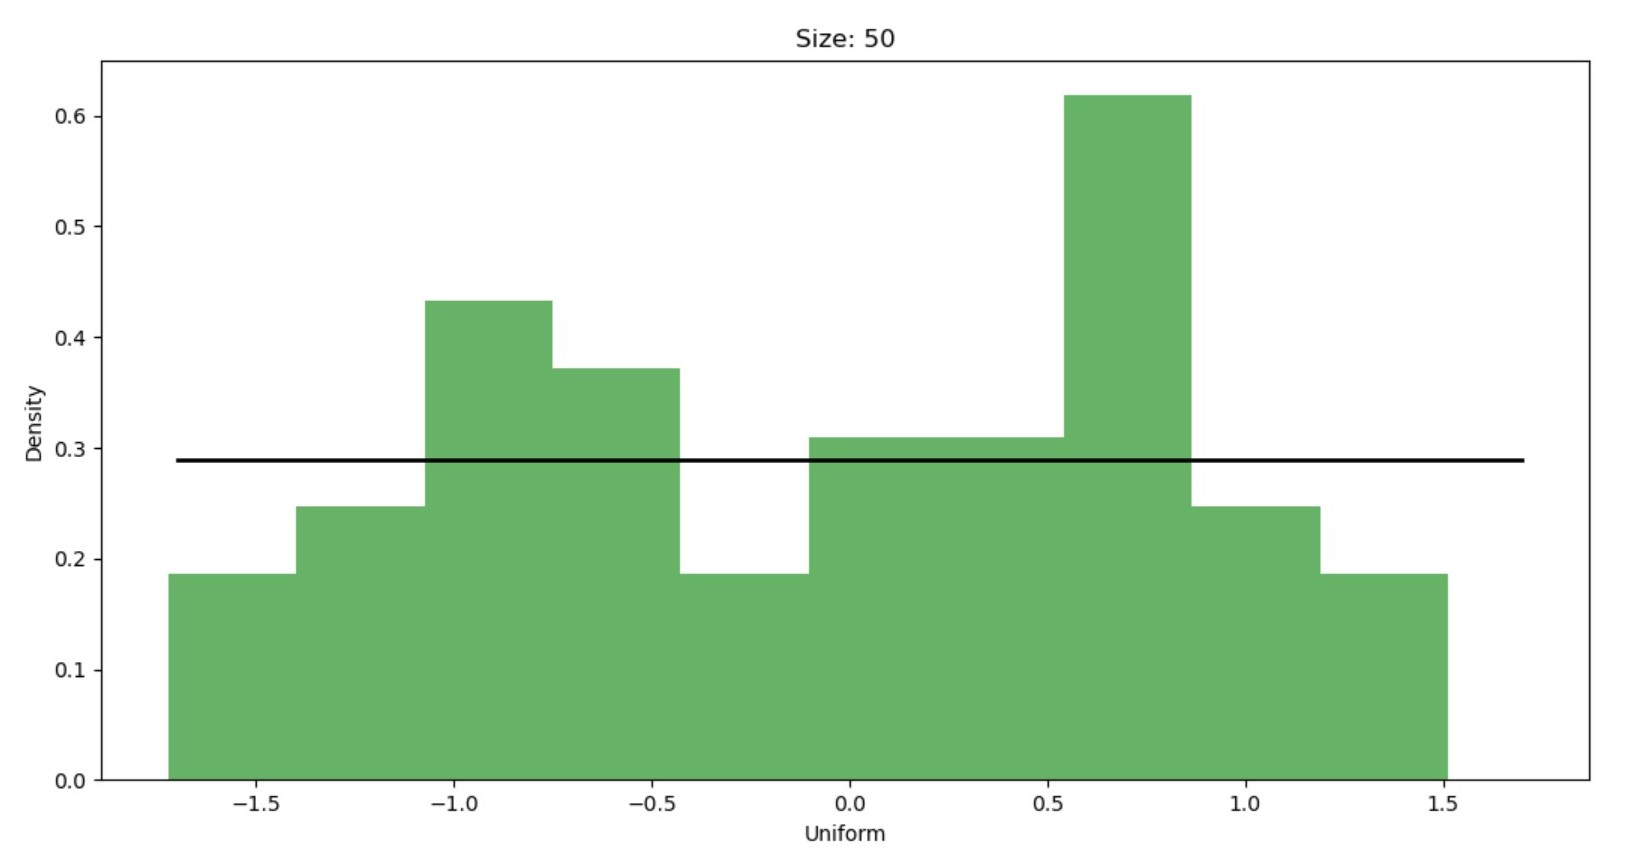
\includegraphics[width=55mm, height =0.25\textheight]{pics/u50.jpg}
		&
		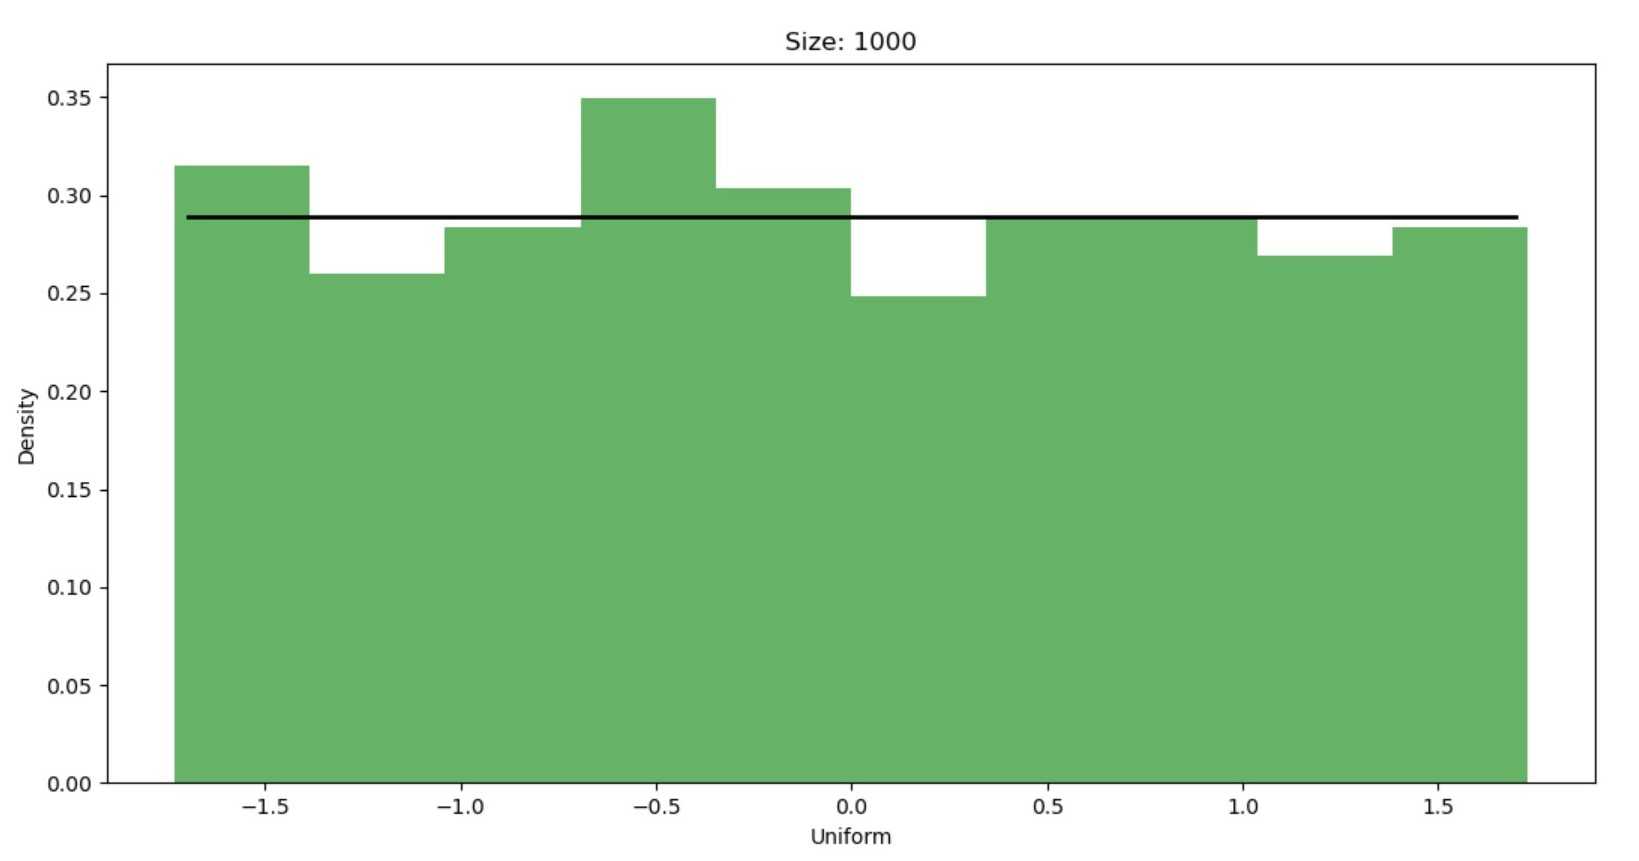
\includegraphics[width=55mm, height =0.25\textheight]{pics/u1000.jpg}
	\end{tabular}
	\caption{Равномерное распределение}
	\label{fig:uniform}
\end{figure}

\subsection{Характеристики положения и рассеяния}
\begin{table}[H]
	\centering
	\begin{tabular}[t]{lrrrrr}
		\hline
		Characteristic   &      Mean &    Median &       $z_R$ &      $z_Q$ &      $z_{tr}$ \\
		\hline
		Normal E(z) 10   &  0.025501 &  0.010119 &  0.030651 & 0.030570 &  0.025708 \\
		Normal D(z) 10   &  0.103765 &  0.092774 &  0.476065 & 0.505294 &  0.172139 \\
		Normal E(z) 100  & 0.001106 & 0.001414  &  -0.04678 & 0.008496 & 0.005806 \\
		Normal D(z) 100  &  0.010594 &  0.009886  &  0.461752 & 0.514966 &  0.018883 \\
		Normal E(z) 1000 & -0.000306 & 0.00014  & 0.029287  & 0.017512 & -0.001402 \\
		Normal D(z) 1000 &  0.0010219 &  0.00090 &  0.499531  & 0.498409 &  0.0020510 \\
		\hline
	\end{tabular}
	\caption{Нормальное распределение}
	\label{tab:normal}
\end{table}

\begin{table}[ht]
	\centering
	\begin{tabular}[t]{lrrrrr}
		\hline
		Characteristic   &        Mean &    Median &            $z_R$ &       $z_Q$ &      $z_{tr}$ \\
		\hline
		Cauchy E(z) 10   &   -1.82930 &  -0.01278 &   -3.6080     &  -0.6565 &  -1.73308 \\
		Cauchy D(z) 10   &  987.1422    &  0.34462 & 8934.589       &  854.6997 &  1708.300 \\
		Cauchy E(z) 100  &   -8.04716  & -0.002323 & 2.58638      & 3.76963 & -17.4805 \\
		Cauchy D(z) 100  & 90333.65   &  0.024408 &    3996.35 &  5978.85 &  359703.9  \\
		Cauchy E(z) 1000 &   0.0993672  & 0.000122 &  -2.16597     &  -0.68649  & -0.033700 \\
		Cauchy D(z) 1000 & 1228.695   &  0.0024604 &    3185.117 &  1023.5756 &  4370.5033 \\
		\hline
	\end{tabular}
	\caption{Распределение Коши}
	\label{tab:cauchy}
\end{table}

\begin{table}[ht]
	\centering
	\begin{tabular}[t]{lrrrrr}
		\hline
		Characteristic    &      Mean &    Median &       $z_R$ &       $z_Q$ &      $z_{tr}$ \\
		\hline
		Laplace E(z) 10   &  -0.006466 &  0.000874 & -0.017804 &  -0.029233 &  -0.010286 \\
		Laplace D(z) 10   &  0.0967693 &  0.068329 &  0.529119 &  0.4894004 &  0.159409 \\
		Laplace E(z) 100  & -0.002621 & -0.002186 & 0.0325949 & 0.000488 & -0.007330 \\
		Laplace D(z) 100  &  0.010093 &  0.006105 &  0.5098014 &  0.528626 &  0.020044 \\
		Laplace E(z) 1000 &  -0.000461 &  4.5834-05 &  0.005827 &  0.008741 &  -0.0003342 \\
		Laplace D(z) 1000 &  0.000950 &  0.000526 &  0.503384 &  0.483016 &  0.001967 \\
		\hline
	\end{tabular}
	\caption{Распределение Лапласа}
	\label{tab:laplace}
\end{table}

\begin{table}[ht]
	\centering
	\begin{tabular}[t]{lrrrrr}
		\hline
		Characteristic    &      Mean &   Median &       $z_R$ &      $z_Q$ &     $z_{tr}$ \\
		\hline
		Poisson E(z) 10   & 10.0305   & 9.887  	 &  9.9375   & 10.1255  & 10.0543     \\
		Poisson D(z) 10   &  1.05715  & 1.45523  &  5.1613   & 5.0939   & 1.70460  \\
		Poisson E(z) 100  & 9.978119   & 9.8255   & 9.8905   & 9.777 & 9.98496  \\
		Poisson D(z) 100  &  0.097413 & 0.1972  &  5.11775 & 5.105771 & 0.198463 \\
		Poisson E(z) 1000 & 10.00179   & 9.997   & 9.905    & 9.988  & 10.0054 \\
		Poisson D(z) 1000 &  0.009803 & 0.001991 &  5.31547 & 5.15535 & 0.018978 \\
		\hline
	\end{tabular}
	
	\caption{Распределение Пуассона}
	\label{tab:poisson}
\end{table}

\begin{table}[ht]
	\centering
	\begin{tabular}[t]{lrrrrr}
		\hline
		Characteristic    &      Mean &    Median &       $z_{R}$ &       $z_Q$ &      $z_{tr}$ \\
		\hline
		Uniform E(z) 10   &  0.017459 &  0.016779 &  0.043340 &  -0.011148 &  0.001145 \\
		Uniform D(z) 10   &  0.098445 &  0.219330 &  0.487425 &  0.5378816 &  0.166308 \\
		Uniform E(z) 100  &  -0.002799 &  -0.00437 &  0.017764 &  0.001040 &  0.002232 \\
		Uniform D(z) 100  &  0.010377 &  0.030492 &  0.443175 &  0.514648 &  0.020929 \\
		Uniform E(z) 1000 & 0.001501 & 0.002397 & -0.033368  & 0.026533 & 0.001575  \\
		Uniform D(z) 1000 &  0.001005 &  0.002988 &  0.5136426   &  0.495917 &  0.002077 \\
		\hline
	\end{tabular}
	\caption{Равномерное распределение}
	\label{tab:uniform}
\end{table}

\subsection{Боксплот Тьюки}
\begin{figure}[H]
	\centering
	\begin{tabular}{ccc}
		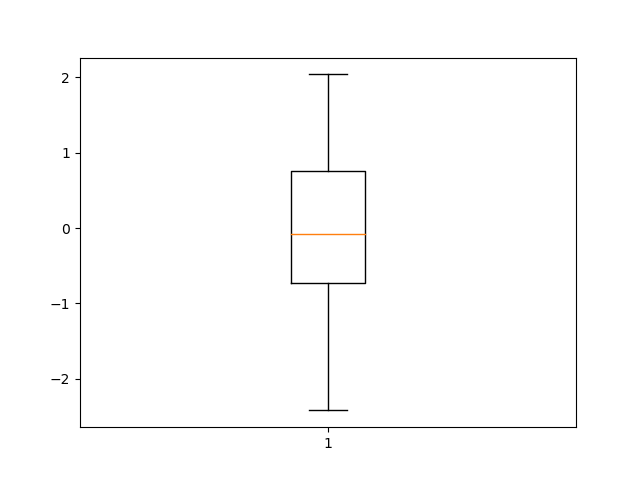
\includegraphics[width=55mm, height =0.25\textheight]{pics/n20.png}
		&
		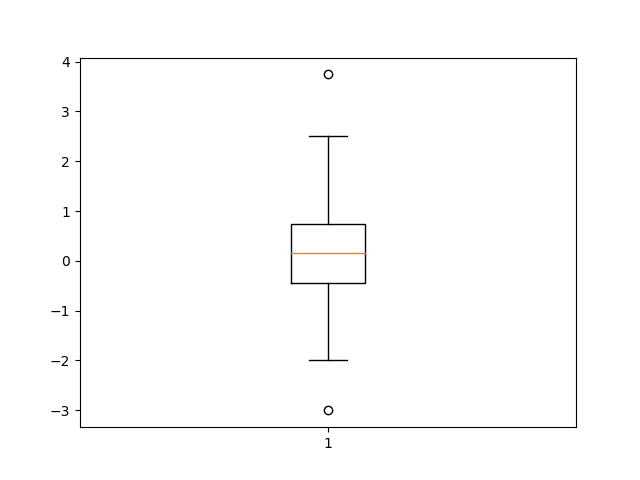
\includegraphics[width=55mm, height =0.25\textheight]{pics/n100.png}
	\end{tabular}
	\caption{Нормальное распределение}
	\label{fig:normal}
\end{figure}

\begin{figure}[H]
	\centering
	\begin{tabular}{ccc}
		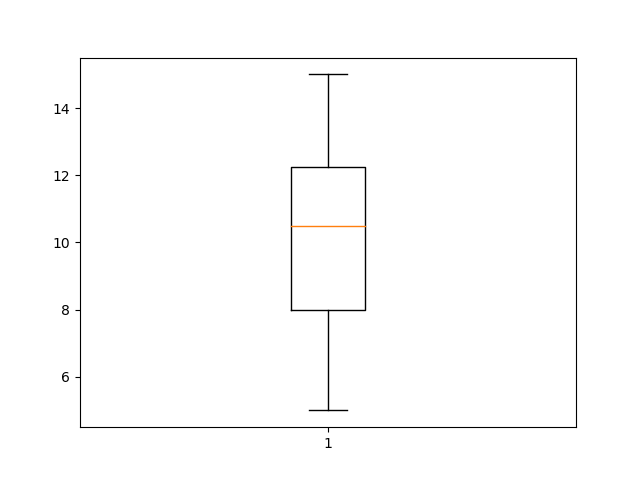
\includegraphics[width=55mm, height =0.25\textheight]{pics/c20.png}
		&
		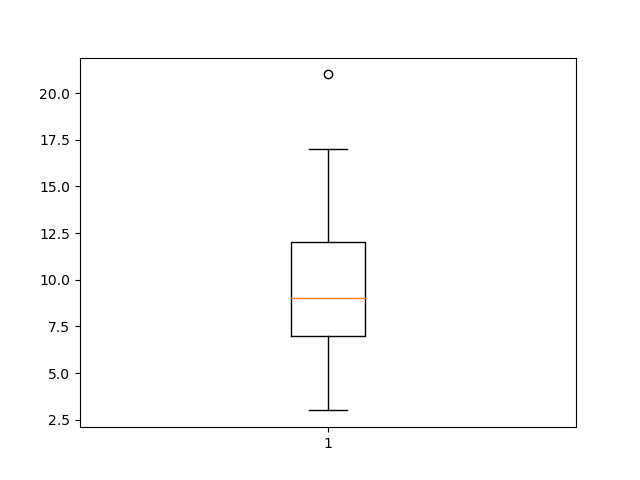
\includegraphics[width=55mm, height =0.25\textheight]{pics/c100.png}\
	\end{tabular}
	\caption{Распределение Коши}
	\label{fig:cauchy}
\end{figure}


\begin{figure}[H]
	\centering
	\begin{tabular}{ccc}
		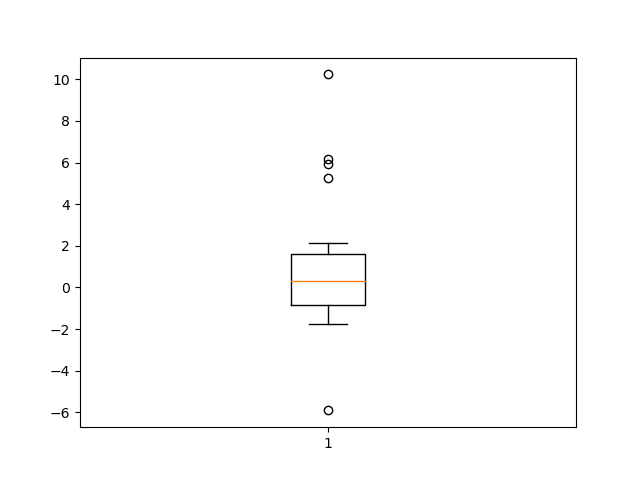
\includegraphics[width=55mm, height =0.25\textheight]{pics/l20.png}
		&
		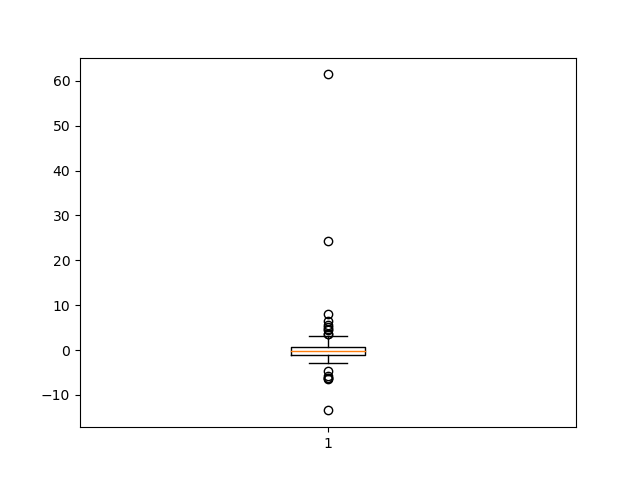
\includegraphics[width=55mm, height =0.25\textheight]{pics/l100.png}\
	\end{tabular}
	\caption{Распределение Лапласа}
	\label{fig:laplace}
\end{figure}


\begin{figure}[H]
	\centering
	\begin{tabular}{ccc}
		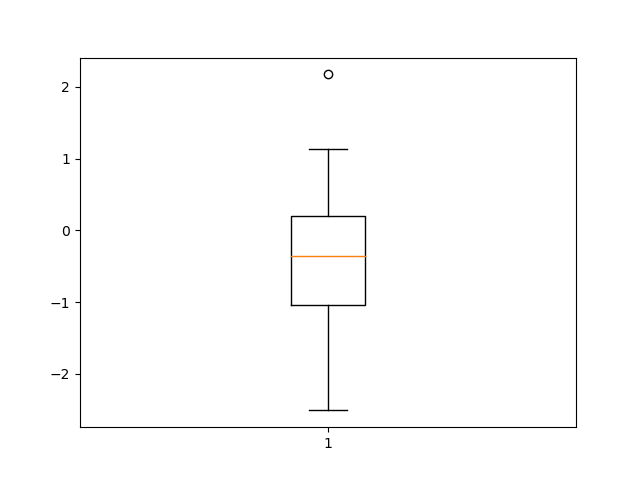
\includegraphics[width=55mm, height =0.25\textheight]{pics/p20.png}
		&
		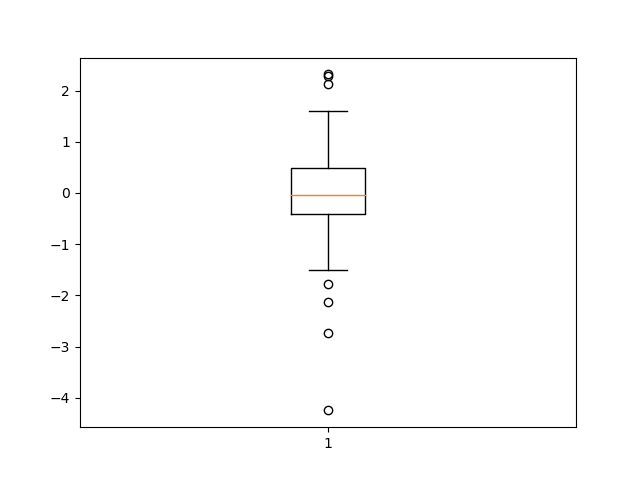
\includegraphics[width=55mm, height =0.25\textheight]{pics/p100.png}
	\end{tabular}
	\caption{Распределение Пуассона}
	\label{fig:poisson}
\end{figure}


\begin{figure}[H]
	\centering
	\begin{tabular}{ccc}
		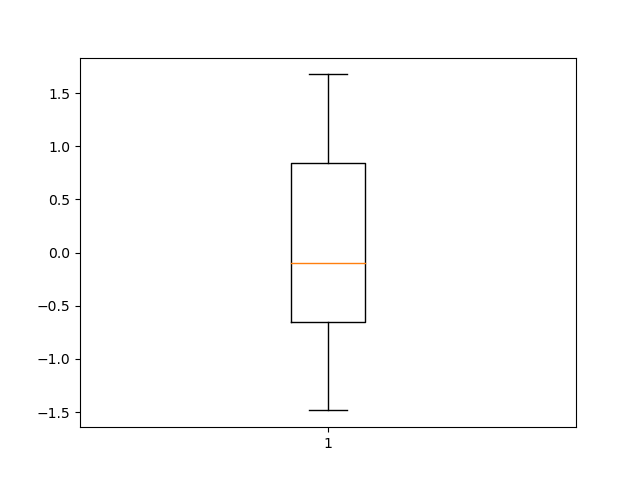
\includegraphics[width=55mm, height =0.25\textheight]{pics/u20.png}
		&
		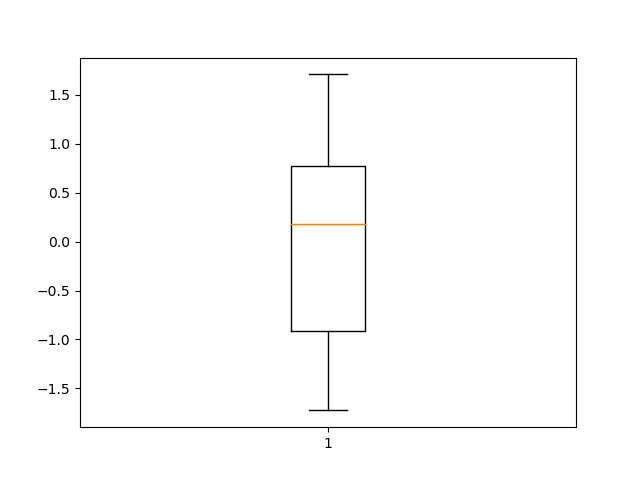
\includegraphics[width=55mm, height =0.25\textheight]{pics/u100.png}
	\end{tabular}
	\caption{Равномерное распределение}
	\label{fig:uniform}
\end{figure}

\subsection{Доля выбросов}
\begin{table}[H]
	\centering
	\begin{tabular}[t]{lr}
		\hline
		Выборка   &      Доля выбросов		\\
		\hline
		Normal n=20   	&	0.06 				\\
		Normal n=100   	&  	0.05		\\
		Cauchy n=20 	& 	0.15  				\\
		Cauchy n=100	&  	0.16 		\\
		Laplace n=20		& 	0.08  			\\
		Laplace n=100	&  	0.07 		\\
		Poisson n=20	&	0.02 				\\
		Poisson n=100	&	0.01 				\\
		Uniform n=20	&	0 				\\
		Uniform n=100	&	0 				\\
		\hline
	\end{tabular}
	\caption{Доля выбросов}
	\label{tab:normal}
\end{table}

\subsection{Теоретическая вероятность выбросов}
\begin{table}[H]
	\centering
	\begin{tabular}[t]{lrrrrr}
		\hline
		Распределение   &      $Q_1^T$	& $Q_3^T$ & $X_1^T$ & $X_2^T$ & $P_B^T$	\\
		\hline
		Нормальное распределение 	& -0.674& 0.674 & -2.698 	&  2.698 	& 0.007 \\
		Распределение Коши 			& -1	& 1		&  -4		& 4			& 0.156 \\
		Распределение Лапласа 		&-0.490	& 0.490	& -1.961	& 1.961		& 0.063\\
		Распределение Пуассона 		& 8		& 12	& 2			& 18		& 0.008 \\
		Равномерное распределение 	&-0.866 & 0.866	& -3.464 	& 3.464 	& 0	\\
		
		\hline
	\end{tabular}
	\caption{Теоретическая вероятность выбросов}
	\label{tab:normal}
\end{table}


\subsection{Эмпирическая функция распределения}
	\begin{figure}[H]
		\centering
		\begin{tabular}{ccc}
			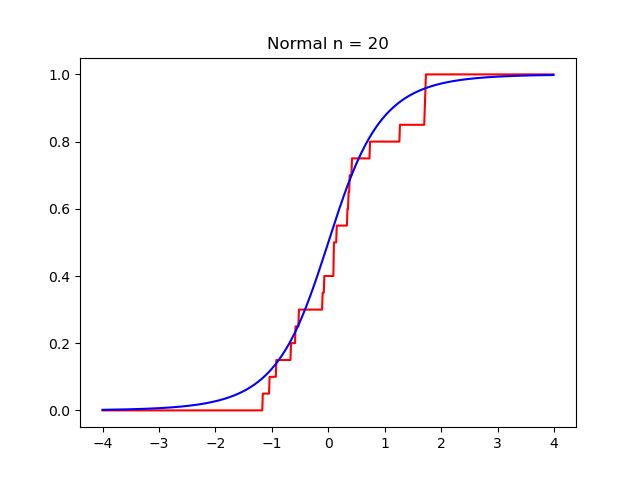
\includegraphics[width=55mm, height =0.25\textheight]{pics/emp_n_20.png}
			&
			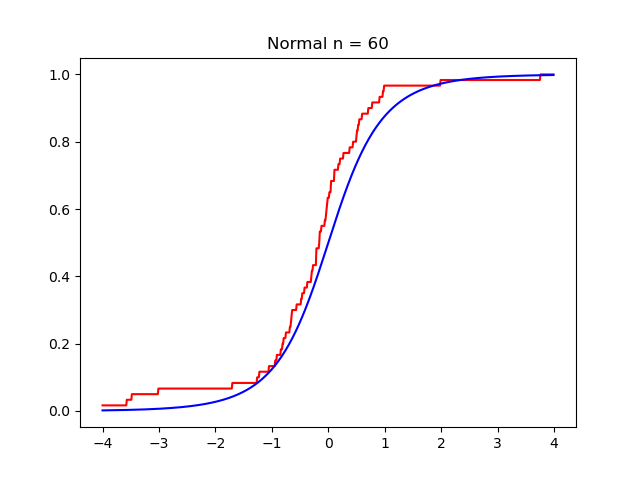
\includegraphics[width=55mm, height =0.25\textheight]{pics/emp_n_60.png}
			&
			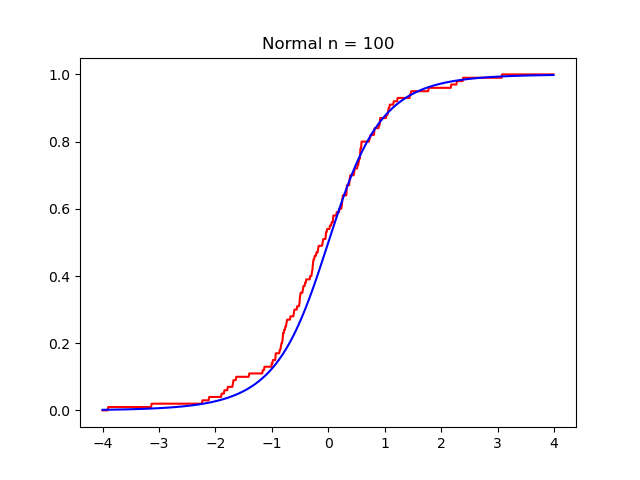
\includegraphics[width=55mm, height =0.25\textheight]{pics/emp_n_100.png}
		\end{tabular}
		\caption{Нормальное распределение}
		\label{fig:normal}
	\end{figure}

	\begin{figure}[H]
		\centering
		\begin{tabular}{ccc}
			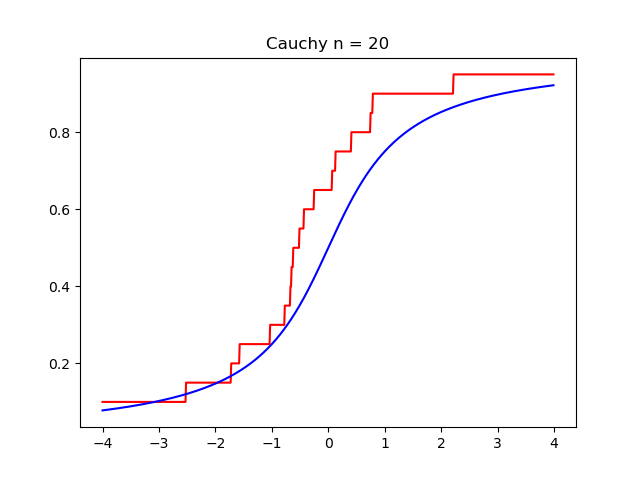
\includegraphics[width=55mm, height =0.25\textheight]{pics/emp_c_20.png}
			&
			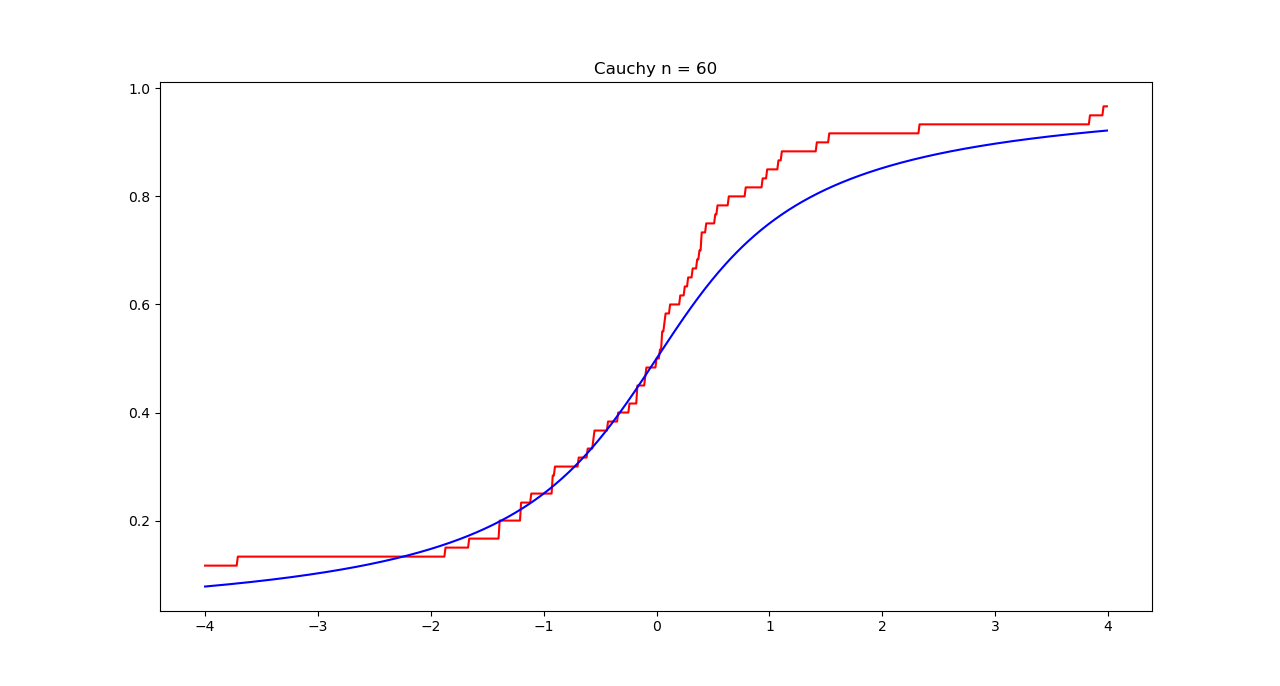
\includegraphics[width=55mm, height =0.25\textheight]{pics/emp_c_60.png}
			&
			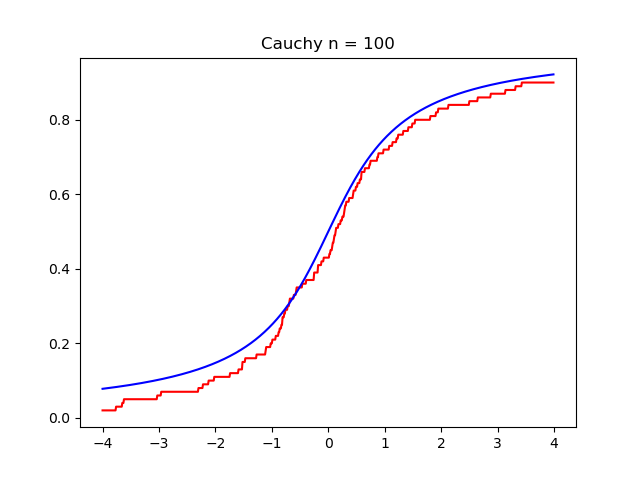
\includegraphics[width=55mm, height =0.25\textheight]{pics/emp_c_100.png}
		\end{tabular}
		\caption{Распределение Коши}
		\label{fig:cauchy}
	\end{figure}
	

	\begin{figure}[H]
		\centering
		\begin{tabular}{ccc}
			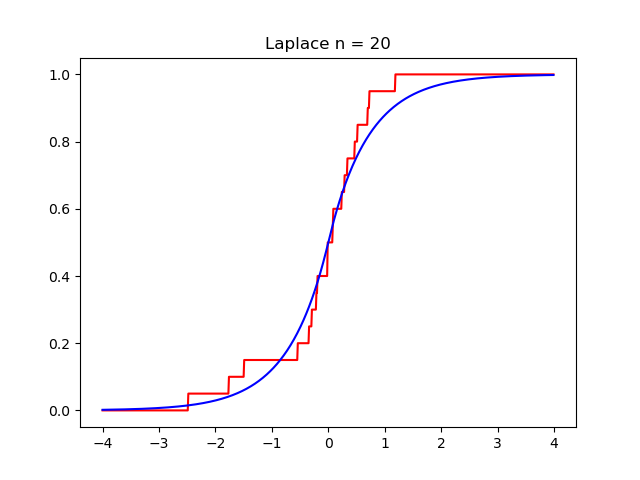
\includegraphics[width=55mm, height =0.25\textheight]{pics/emp_l_20.png}
			&
			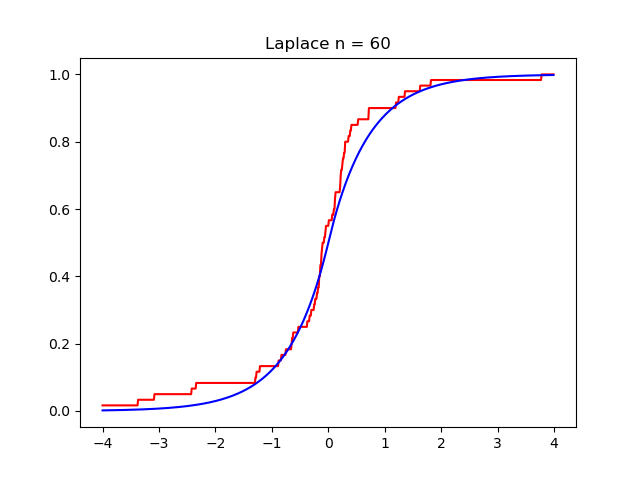
\includegraphics[width=55mm, height =0.25\textheight]{pics/emp_l_60.png}
			&
			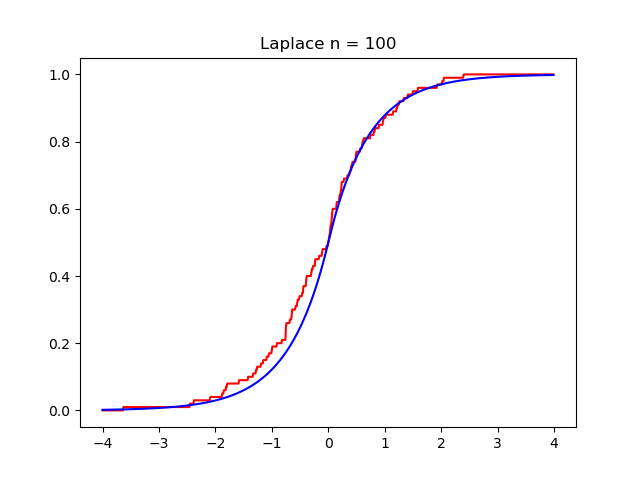
\includegraphics[width=55mm, height =0.25\textheight]{pics/emp_l_100.png}
		\end{tabular}
		\caption{Распределение Лапласа}
		\label{fig:laplace}
	\end{figure}


	\begin{figure}[H]
		\centering
		\begin{tabular}{ccc}
			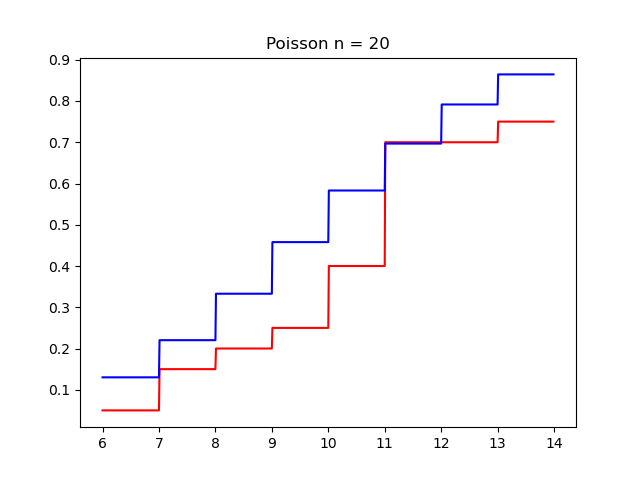
\includegraphics[width=55mm, height =0.25\textheight]{pics/emp_p_20.png}
			&
			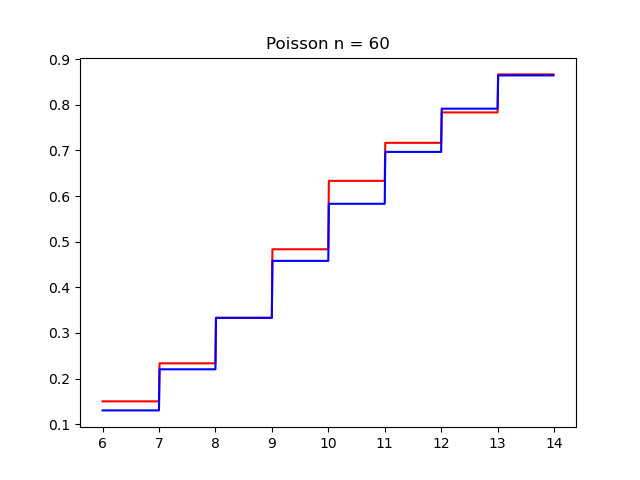
\includegraphics[width=55mm, height =0.25\textheight]{pics/emp_p_60.png}
			&
			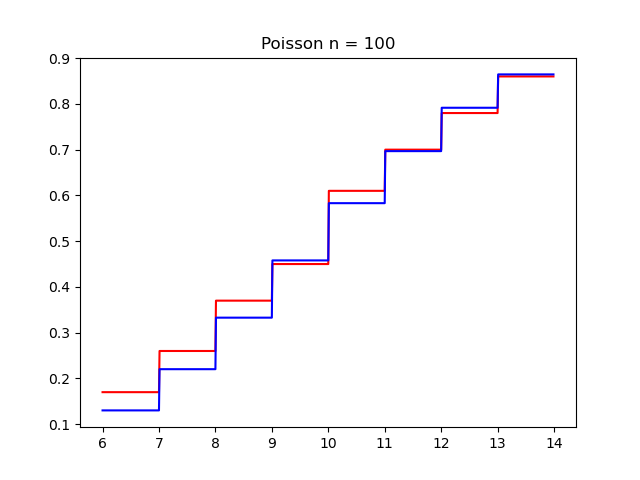
\includegraphics[width=55mm, height =0.25\textheight]{pics/emp_p_100.png}
		\end{tabular}
		\caption{Распределение Пуассона}
		\label{fig:poisson}
	\end{figure}


	\begin{figure}[H]
		\centering
		\begin{tabular}{ccc}
			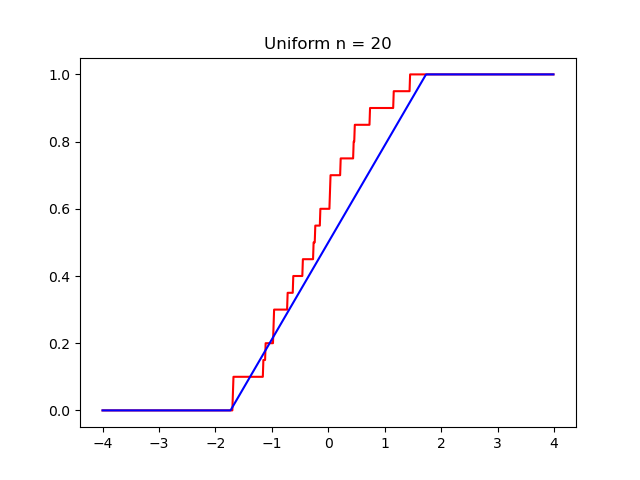
\includegraphics[width=55mm, height =0.25\textheight]{pics/emp_u_20.png}
			&
			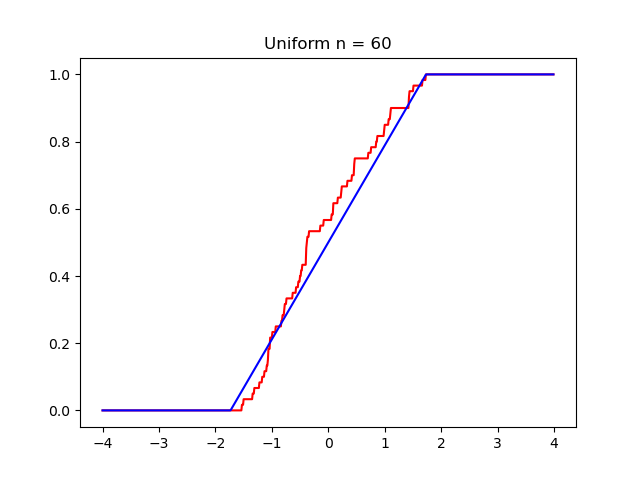
\includegraphics[width=55mm, height =0.25\textheight]{pics/emp_u_60.png}
			&
			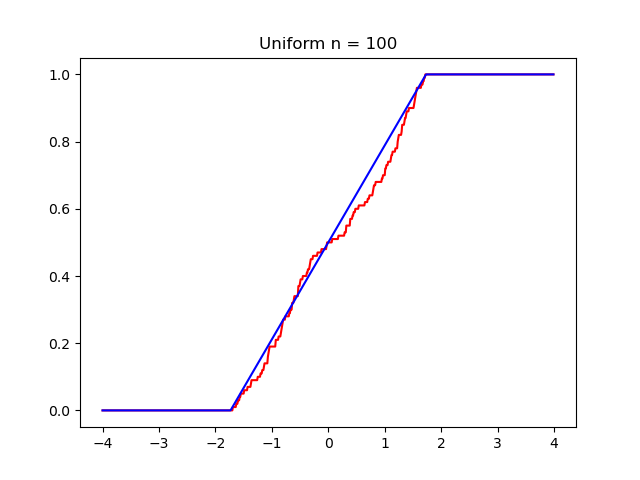
\includegraphics[width=55mm, height =0.25\textheight]{pics/emp_u_100.png}
		\end{tabular}
		\caption{Равномерное распределение}
		\label{fig:uniform}
	\end{figure}

\subsection{Ядерные оценки плотности распределения}
	\begin{figure}[H]
		\centering
			\begin{tabular}{ccc}
			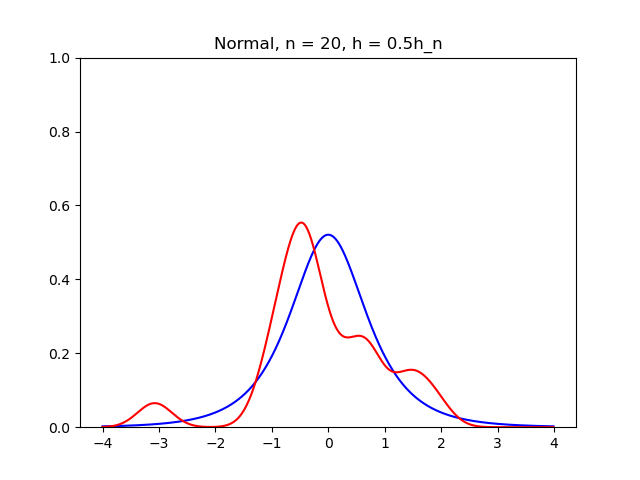
\includegraphics[width=55mm, height =0.25\textheight]{pics/ker_n_20_1.png}
			&
			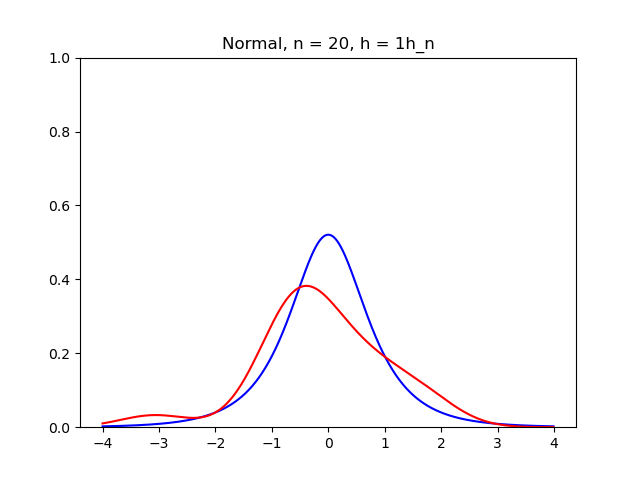
\includegraphics[width=55mm, height =0.25\textheight]{pics/ker_n_20_2.png}
			&
			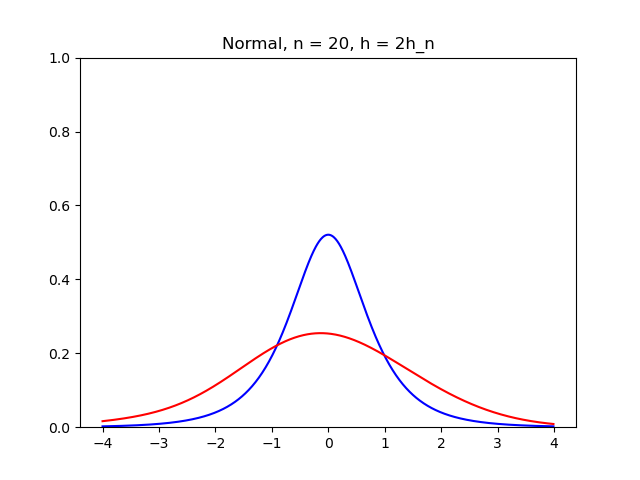
\includegraphics[width=55mm, height =0.25\textheight]{pics/ker_n_20_3.png}
			\end{tabular}
		\caption{Нормальное распределение, $n = 20$}
		\label{fig:normal}
	\end{figure}

	\begin{figure}[H]
		\centering
		\begin{tabular}{ccc}
			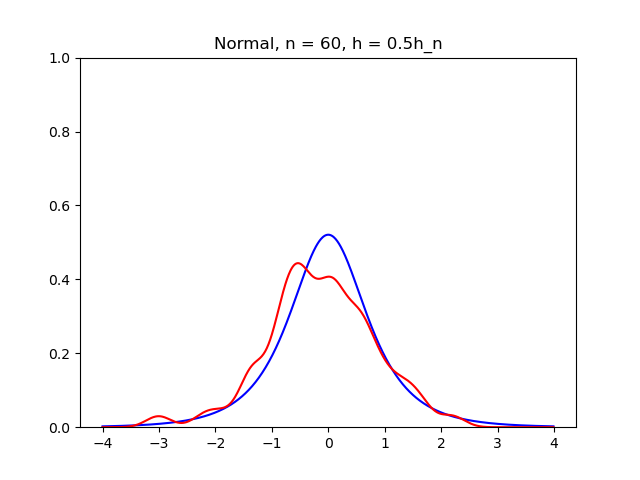
\includegraphics[width=55mm, height =0.25\textheight]{pics/ker_n_60_1.png}
			&
			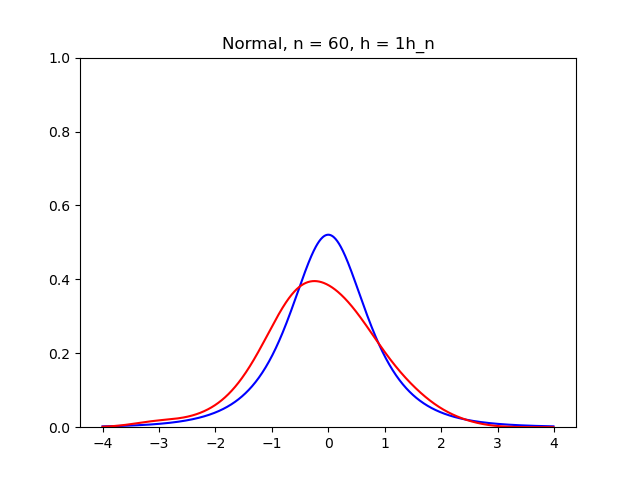
\includegraphics[width=55mm, height =0.25\textheight]{pics/ker_n_60_2.png}
			&
			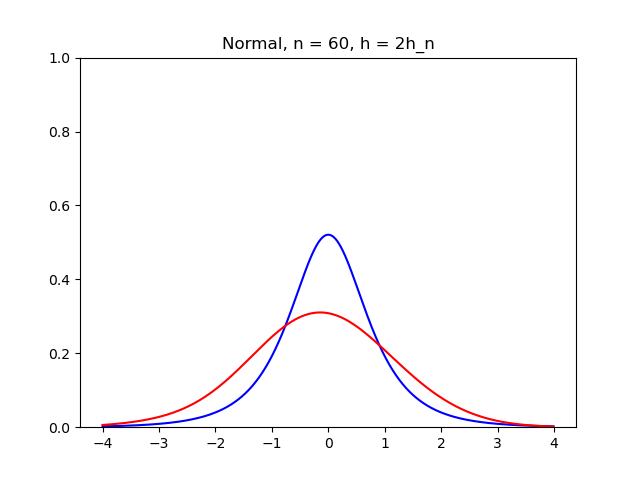
\includegraphics[width=55mm, height =0.25\textheight]{pics/ker_n_60_3.png}
		\end{tabular}
		\caption{Нормальное распределение, $n = 60$}
		\label{fig:normal}
	\end{figure}

	\begin{figure}[H]
		\centering
		\begin{tabular}{ccc}
			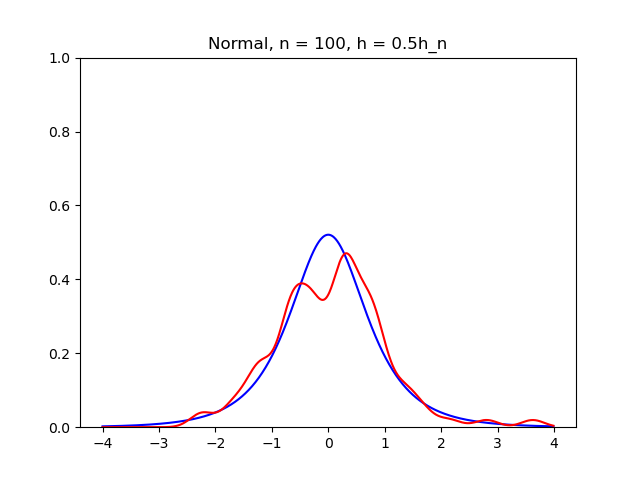
\includegraphics[width=55mm, height =0.25\textheight]{pics/ker_n_100_1.png}
			&
			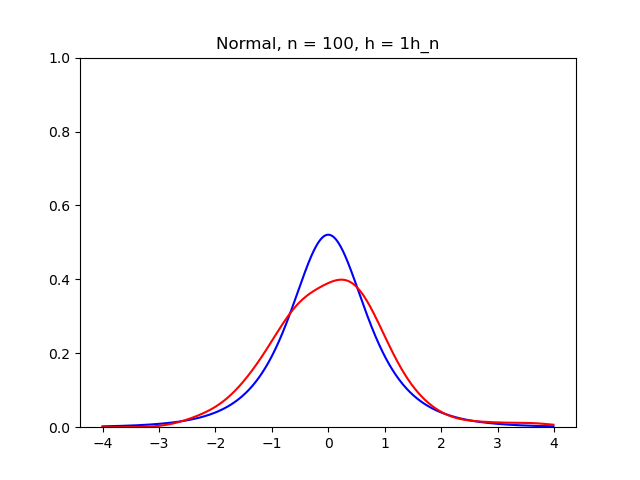
\includegraphics[width=55mm, height =0.25\textheight]{pics/ker_n_100_2.png}
			&
			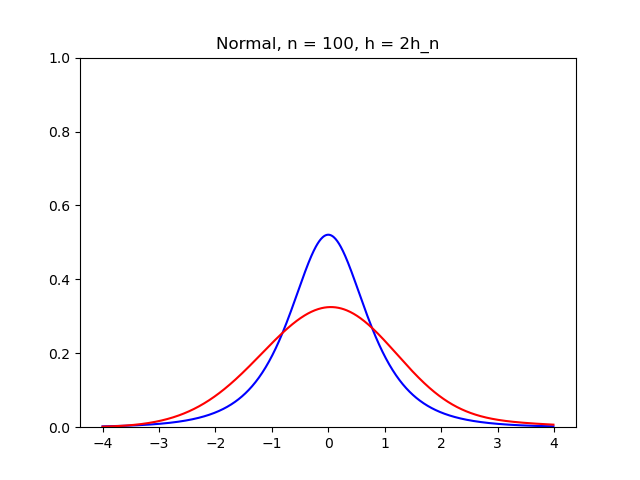
\includegraphics[width=55mm, height =0.25\textheight]{pics/ker_n_100_3.png}
		\end{tabular}
		\caption{Нормальное распределение, $n = 100$}
		\label{fig:normal}
	\end{figure}
	
	\begin{figure}[H]
		\centering
		\begin{tabular}{ccc}
			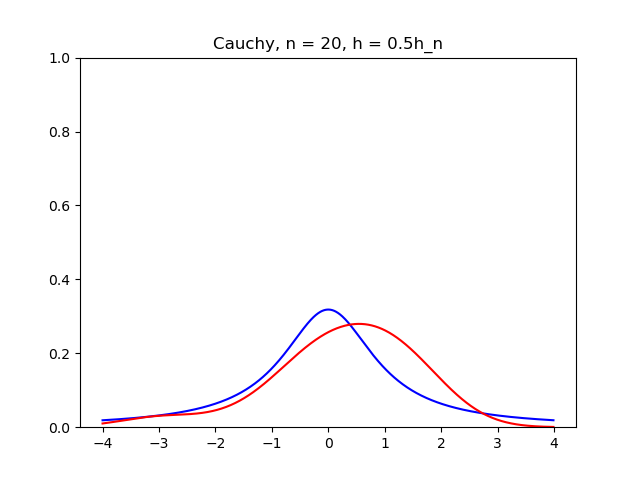
\includegraphics[width=55mm, height =0.25\textheight]{pics/ker_c_20_1.png}
			&
			\includegraphics[width=55mm, height =0.25\textheight]{pics/ker_c_20_2.png}
			&
			\includegraphics[width=55mm, height =0.25\textheight]{pics/ker_c_20_3.png}
		\end{tabular}
		\caption{Распределение Коши, $n = 20$}
		\label{fig:cauchy}
	\end{figure}

	\begin{figure}[H]
		\centering
		\begin{tabular}{ccc}
			\includegraphics[width=55mm, height =0.25\textheight]{pics/ker_c_60_1.png}
			&
			\includegraphics[width=55mm, height =0.25\textheight]{pics/ker_c_60_2.png}
			&
			\includegraphics[width=55mm, height =0.25\textheight]{pics/ker_c_60_3.png}
		\end{tabular}
		\caption{Распределение Коши, $n = 60$}
		\label{fig:cauchy}
	\end{figure}

	\begin{figure}[H]
		\centering
		\begin{tabular}{ccc}
			\includegraphics[width=55mm, height =0.25\textheight]{pics/ker_c_100_1.png}
			&
			\includegraphics[width=55mm, height =0.25\textheight]{pics/ker_c_100_2.png}
			&
			\includegraphics[width=55mm, height =0.25\textheight]{pics/ker_c_100_3.png}
		\end{tabular}
		\caption{Распределение Коши, $n = 100$}
		\label{fig:cauchy}
	\end{figure}
	
	
	\begin{figure}[H]
		\centering
		\begin{tabular}{ccc}
			\includegraphics[width=55mm, height =0.25\textheight]{pics/ker_l_20_1.png}
			&
			\includegraphics[width=55mm, height =0.25\textheight]{pics/ker_l_20_2.png}
			&
			\includegraphics[width=55mm, height =0.25\textheight]{pics/ker_l_20_3.png}
		\end{tabular}
		\caption{Распределение Лапласа, $n = 20$}
		\label{fig:laplace}
	\end{figure}

	\begin{figure}[H]
		\centering
		\begin{tabular}{ccc}
			\includegraphics[width=55mm, height =0.25\textheight]{pics/ker_l_60_1.png}
			&
			\includegraphics[width=55mm, height =0.25\textheight]{pics/ker_l_60_2.png}
			&
			\includegraphics[width=55mm, height =0.25\textheight]{pics/ker_l_60_3.png}
		\end{tabular}
		\caption{Распределение Лапласа, $n = 60$}
		\label{fig:laplace}
	\end{figure}

	\begin{figure}[H]
		\centering
		\begin{tabular}{ccc}
			\includegraphics[width=55mm, height =0.25\textheight]{pics/ker_l_100_1.png}
			&
			\includegraphics[width=55mm, height =0.25\textheight]{pics/ker_l_100_2.png}
			&
			\includegraphics[width=55mm, height =0.25\textheight]{pics/ker_l_100_3.png}
		\end{tabular}
		\caption{Распределение Лапласа, $n = 100$}
		\label{fig:laplace}
	\end{figure}
	
	
	\begin{figure}[H]
		\centering
		\begin{tabular}{ccc}
			\includegraphics[width=55mm, height =0.25\textheight]{pics/ker_p_20_1.png}
			&
			\includegraphics[width=55mm, height =0.25\textheight]{pics/ker_p_20_2.png}
			&
			\includegraphics[width=55mm, height =0.25\textheight]{pics/ker_p_20_3.png}
		\end{tabular}
		\caption{Распределение Пуассона, $n = 20$}
		\label{fig:poisson}
	\end{figure}

	\begin{figure}[H]
		\centering
		\begin{tabular}{ccc}
			\includegraphics[width=55mm, height =0.25\textheight]{pics/ker_p_60_1.png}
			&
			\includegraphics[width=55mm, height =0.25\textheight]{pics/ker_p_60_2.png}
			&
			\includegraphics[width=55mm, height =0.25\textheight]{pics/ker_p_60_3.png}
		\end{tabular}
		\caption{Распределение Пуассона, $n = 60$}
		\label{fig:poisson}
	\end{figure}

	\begin{figure}[H]
		\centering
		\begin{tabular}{ccc}
			\includegraphics[width=55mm, height =0.25\textheight]{pics/ker_p_100_1.png}
			&
			\includegraphics[width=55mm, height =0.25\textheight]{pics/ker_p_100_2.png}
			&
			\includegraphics[width=55mm, height =0.25\textheight]{pics/ker_p_100_3.png}
		\end{tabular}
		\caption{Распределение Пуассона, $n = 100$}
		\label{fig:poisson}
	\end{figure}
	
	
	\begin{figure}[H]
		\centering
		\begin{tabular}{ccc}
			\includegraphics[width=55mm, height =0.25\textheight]{pics/ker_u_20_1.png}
			&
			\includegraphics[width=55mm, height =0.25\textheight]{pics/ker_u_20_2.png}
			&
			\includegraphics[width=55mm, height =0.25\textheight]{pics/ker_u_20_3.png}
		\end{tabular}
		\caption{Равномерное распределение, $n = 20$}
		\label{fig:uniform}
	\end{figure}


	\begin{figure}[H]
	\centering
	\begin{tabular}{ccc}
		\includegraphics[width=55mm, height =0.25\textheight]{pics/ker_u_60_1.png}
		&
		\includegraphics[width=55mm, height =0.25\textheight]{pics/ker_u_60_2.png}
		&
		\includegraphics[width=55mm, height =0.25\textheight]{pics/ker_u_60_3.png}
	\end{tabular}
	\caption{Равномерное распределение, $n = 60$}
	\label{fig:uniform}
	\end{figure}

	\begin{figure}[H]
	\centering
	\begin{tabular}{ccc}
		\includegraphics[width=55mm, height =0.25\textheight]{pics/ker_u_100_1.png}
		&
		\includegraphics[width=55mm, height =0.25\textheight]{pics/ker_u_100_2.png}
		&
		\includegraphics[width=55mm, height =0.25\textheight]{pics/ker_u_100_3.png}
	\end{tabular}
	\caption{Равномерное распределение, $n = 100$}
	\label{fig:uniform}
	\end{figure}
	
